\documentclass[11pt]{article}
\usepackage[a4paper,margin=25mm]{geometry}
\usepackage{amsmath,amssymb,amsthm,mathtools,booktabs,array}
\usepackage[dvipsnames]{xcolor}
\usepackage{graphicx,hyperref,fancyhdr}
\hypersetup{hypertexnames=false,colorlinks=true,linkcolor=MidnightBlue,
 citecolor=MidnightBlue,urlcolor=MidnightBlue,
 pdftitle={A packing-dimension condition for positive pinned distances}}
\setlength{\parindent}{0pt}
\setlength{\parskip}{5pt}
\setlength{\emergencystretch}{2em}
\setlength{\headheight}{14pt}
\pagestyle{fancy}\fancyhf{}
\fancyhead[L]{\small A packing condition for pinned distances}
\fancyhead[R]{\small 30 September 2026}\fancyfoot[C]{\thepage}
\newtheorem{theorem}{Theorem}[section]
\newtheorem{proposition}[theorem]{Proposition}
\newtheorem{lemma}[theorem]{Lemma}
\theoremstyle{definition}\newtheorem{remark}[theorem]{Remark}
\newcommand{\R}{\mathbb R}
\newcommand{\HH}{\dim_{\mathrm H}}\newcommand{\PP}{\dim_{\mathrm P}}
\newcommand{\supp}{\operatorname{supp}}\newcommand{\dist}{\operatorname{dist}}
\newcommand{\dd}{\,d}\newcommand{\norm}[1]{\left\|#1\right\|}
\newcommand{\eps}{\varepsilon}

\begin{document}
\begin{center}
{\LARGE\bfseries A packing-dimension condition\\[4pt]
for positive pinned distances}\par
\vspace{5pt}
{\large The theorem, its meaning, and a focused proof}\par
\vspace{3pt}
30 September 2026
\end{center}

\section{The result}
Fix a point \(y\) of a planar set \(E\). Its \emph{pinned distance set} is
\[
 \Delta_y(E)=\{|x-y|:x\in E\}.
\]
The question is whether these distances occupy positive length on the real
line. Write \(d=\HH E\) and \(D=\PP E\). Hausdorff dimension supplies
a measure that does not concentrate too much in small balls; packing
dimension controls the number of small squares needed after restricting
to a suitable part of the set.

\begin{theorem}\label{human:target}
Let \(E\subset\R^2\) be Borel. If
\[
 1<d=\HH E\le\frac54,\qquad \PP E<B_{\rm H}(d),
\]
then there is a point \(y\in E\) such that
\(\mathcal L^1(\Delta_y(E))>0\).
\end{theorem}

The sufficient boundary is
\begin{equation}\label{human:curve}
 B_{\rm H}(d)=
 \begin{cases}
  2d-1,&1<d\le d_\alpha,\\[5pt]
  1+r_2(d-1),&d_\alpha<d\le d_c,\\[5pt]
  \dfrac1{3-2d},&d_c<d\le\dfrac54,
 \end{cases}
\end{equation}
where
\[
 d_\alpha=\frac{7-\sqrt7}{4}\approx1.088562172,
 \qquad d_c=\frac{2+\sqrt6}{4}\approx1.112372436,
\]
and the short middle branch is given explicitly by
\begin{equation}\label{human:root}
 r_2(a)=\frac{6a}
 {2-a+8a^2+\sqrt{4-28a-63a^2+32a^3+64a^4}}.
\end{equation}
The radical is real throughout the required interval, and both joins are
continuous; Appendix~\ref{humanprofile:section} proves these facts.

The packing inequality is \emph{strict}. At \(d=5/4\) it permits
\(D<2\), but does not include \(D=2\). For \(d>5/4\), the theorem of
Guth--Iosevich--Ou--Wang already gives a positive-length pinned distance set
without a packing restriction \cite{giow}. No necessity or global optimality
claim is made for \eqref{human:curve}.

\clearpage
\section{How to read the bound}
For most of the improved range, the formula is simply
\(B_{\rm H}(d)=1/(3-2d)\). The radical only joins this branch to
\(2d-1\) on the small interval between approximately \(1.0886\) and
\(1.1124\).

\begin{center}
\begin{tabular}{lll}
\toprule
Hausdorff dimension \(d\) & Sufficient packing restriction & An allowed value \\
\midrule
\(1.05\) & \(D<1.10\) & \(D=1.08\) \\
\(1.10\) & \(D<28/23\approx1.21739\) & \(D=1.21\) \\
\(1.15\) & \(D<10/7\approx1.42857\) & \(D=1.40\) \\
\(1.20\) & \(D<5/3\approx1.66667\) & \(D=1.60\) \\
\(1.24\) & \(D<25/13\approx1.92308\) & \(D=1.90\) \\
\(1.25\) & \(D<2\) & \(D=1.99\) \\
\bottomrule
\end{tabular}
\end{center}

\begin{figure}[h]
\centering
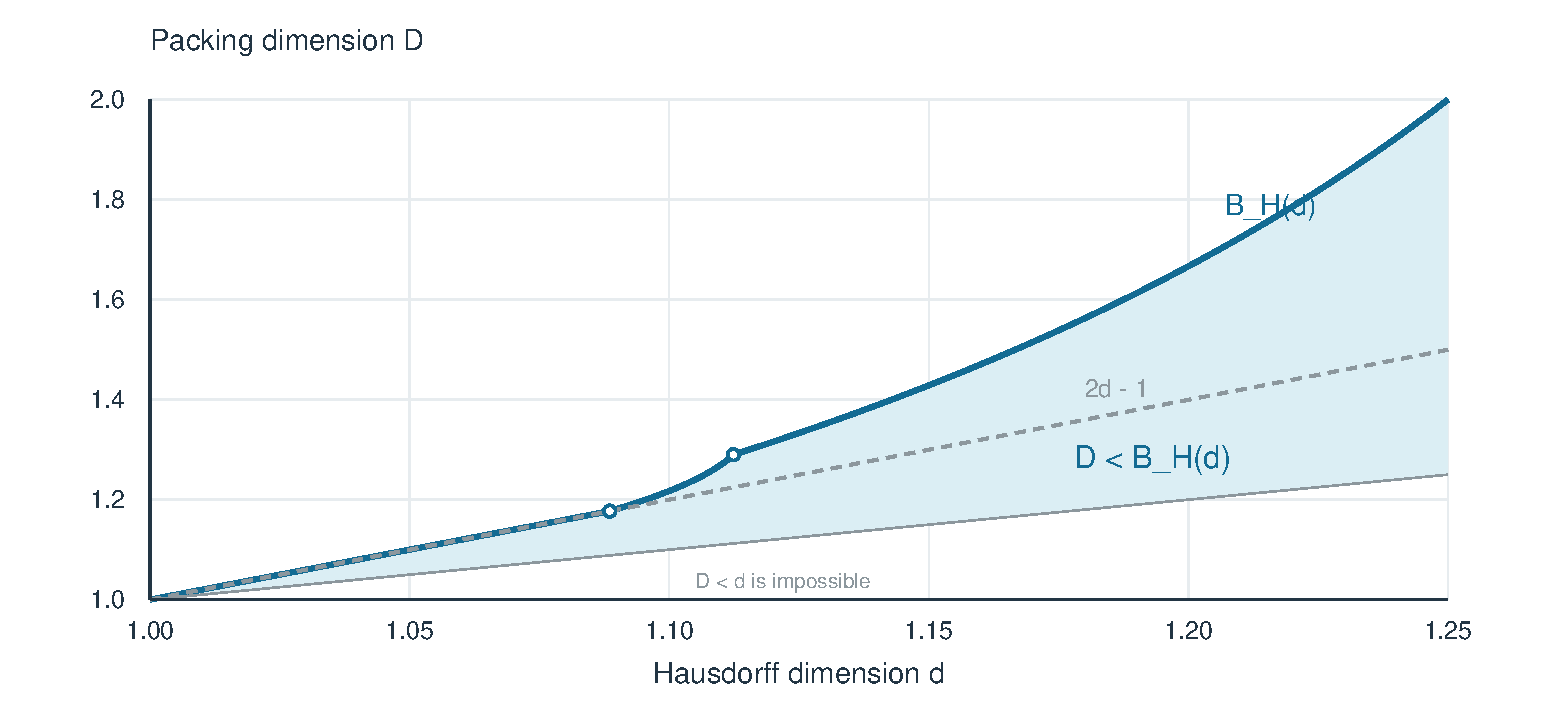
\includegraphics[width=\textwidth]{../figures/falconer-human-curve.pdf}
\caption{The shaded region \(d\le D<B_{\rm H}(d)\) is covered by the
theorem. Its upper boundary is excluded. The dashed line shows the simpler
condition \(D<2d-1\). The graph illustrates the formulas; it is not used
as evidence for the inequalities.}
\end{figure}

For example, at \(d=1.24\), the simpler condition requires \(D<1.48\),
whereas the theorem permits \(D<25/13\). The pin is a point of the original
set, not a point chosen elsewhere in the plane.

\section{The idea of the proof}
Choose a probability \(\mu\) on one compact part of \(E\), and a probability
\(\nu\) on another, separated compact part. The distance distribution from
a pin \(y\) is the pushforward
\[
 (d_y)_*\mu,\qquad d_y(x)=|x-y|.
\]
It suffices to prove that this probability has a Lebesgue density for
\(\nu\)-almost every pin. Such a density has integral one, so its supporting
distance set cannot have zero length.

The proof supplies this density in two regimes. Under \(D<2d-1\), replace
distance by its tangent affine map in small source squares. The resulting
positive densities converge in \(L^1\): their average absolute differences
are summable. Outside that regime, split the source into frequency annuli.
In each annulus discard a small \(L^1\) error and prove a summable
\(L^2\) bound for the remaining density.

The second argument is where the improved curve comes from. The pin measure's
mass distribution across scales is encoded by a Lipschitz function. Rather
than fixing the same intermediate scales for every distribution, choose a
short chain of scales adapted to that function. A one-dimensional calculation
bounds the total loss along the chain. If this loss is smaller than \(d-1\),
the annular density estimates are summable.

Thus the proof has three separate tasks: extract compact measures, bound a
scalar scale-selection problem, and turn that bound into a density. The
remainder of the main text states their precise interfaces and assembles them.
The appendices provide their proofs without the exploratory material from the
longer research manuscript.

\section{A precise proof of the theorem}
\subsection{Measures and compact reduction}
A probability \(\lambda\) is \(t\)-Frostman when
\(\lambda(B(x,r))\le C r^t\) for \(0<r\le1\). Define
\[
 I_s(\lambda)=\iint|x-x'|^{-s}\dd\lambda(x)\dd\lambda(x').
\]
On a bounded support, the Frostman estimate implies \(I_s(\lambda)<\infty\)
for every \(0<s<t\), by summing the concentric distance annuli.
Let \(N(K,r)\) be the least number of radius-\(r\) balls covering \(K\).

\begin{lemma}[Compact measures with the required exponents]
\label{human:compact}
If \(E\) is Borel, \(0<t<\HH E\), and \(\PP E<u\), there are separated
compact sets inside \(E\) carrying \(t\)-Frostman probabilities \(\mu,\nu\)
such that each support has covering number at most \(Cr^{-u}\).
\end{lemma}
\begin{proof}
Frostman's lemma supplies a compactly supported \(t\)-Frostman probability
on \(E\). The countable-cover characterization of packing dimension covers
\(E\) by bounded sets of upper box dimension strictly below \(u\).
Taking closures and intersecting with \(E\) makes this a Borel cover without
changing the upper box bounds. One member has positive Frostman mass.
Inner regularity gives a compact subset of positive mass in it; its covering
numbers are bounded by \(Cr^{-u}\). The restricted measure is nonatomic,
so choose two disjoint small closed balls, a positive distance apart, whose
intersections with that compact set have positive mass. Normalize the two
restrictions. The Frostman and covering bounds persist, with new constants.
\end{proof}

\subsection{The two density estimates}
\begin{proposition}[The direct comparison]
\label{human:coherent-interface}
Suppose separated compact probabilities \(\mu,\nu\) are \(t\)-Frostman,
where \(1<s<\min\{t,2\}\), and \(N(\supp\mu,r)\le Cr^{-u}\).
If \(u<2s-1\), then \((d_y)_*\mu\) is absolutely continuous for
\(\nu\)-almost every \(y\).
\end{proposition}
The proof in Appendix~\ref{human:coherent-section} constructs the positive
affine approximations described above and proves their \(L^1\) convergence.

Here is the interface for the improved branch. For a 1-Lipschitz profile
\(g:[0,N]\to\R\), the cost of an edge from \(n\) down to \(m<n\) is
\[
 c_g(m,n)=g(m)-\min_{m\le x\le n}g(x).
\]
The edge is permitted when \(2n-m\le N\). Its cost records a possible
loss caused by concentration between those two scales.

\begin{proposition}[The profile-to-density implication]
\label{human:transfer}
Suppose separated compact probabilities \(\mu,\nu\) are \(t\)-Frostman,
where \(1<s<t\), and \(N(\supp\nu,r)\le Cr^{-u}\), with \(s<u<2\).
Suppose there is a number \(\mathcal C<s-1\) with the following property.

Every piecewise affine, 1-Lipschitz profile satisfying
\[
 g(0)=0,\qquad (s-1)x\le g(x)\le(u-1)x
\]
has a permitted chain from \(n_0=(1-\zeta)N\) to zero whose total cost is
at most \(\mathcal C N\), allowing an arbitrarily small additional
multiple of \(N\). The number of edges is bounded in terms of
\(\zeta>0\), independently of \(N\) and the profile. Rounding to a grid
of mesh \(T\) and allowing additive barrier errors of size \(\epsilon N\)
changes the bound by at most \(C K(\epsilon N+T)\), where \(K\) is the
chain length.

Then \((d_y)_*\mu\) is absolutely continuous for \(\nu\)-almost every pin.
\end{proposition}
Appendix~\ref{human:analytic-proof} proves this implication, including the
finite measure regularization, deletion estimate, Fourier iteration, and
identification of the limiting density. Appendix~\ref{uf:embedding} proves
the one-step Fourier estimate used there.

The real-variable calculation in Appendix~\ref{humanprofile:section}
establishes exactly the following sufficient input:
\begin{equation}\label{human:scalar-interface}
 1<s\le\frac54,\quad 2s-1\le u<B_{\rm H}(s)
 \quad\Longrightarrow\quad
 \text{the profile bound holds with some }\mathcal C<s-1.
\end{equation}
That calculation also proves continuity of \(B_{\rm H}\), so all exponent
choices in the next paragraph are justified by strict inequalities.

\subsection{Assembly}
\begin{proof}[Proof of Theorem~\ref{human:target}]
If \(D<2d-1\), choose \(1<s<t<d\) and \(D<u<2s-1\).
Lemma~\ref{human:compact} gives the two compact probabilities, and
Proposition~\ref{human:coherent-interface} gives their pinned densities.

Otherwise \(2d-1\le D<B_{\rm H}(d)\). Continuity and strictness allow
\(s<d\), sufficiently close to \(d\), and then \(t,u\) such that
\[
 1<s<t<d,\qquad D<u<B_{\rm H}(s),\qquad 2s-1<u<2.
\]
When \(d=5/4\), choose \(s<5/4\); the strict condition \(D<2\) still
provides the required room. Apply Lemma~\ref{human:compact}.
Equation~\eqref{human:scalar-interface} and
Proposition~\ref{human:transfer} give absolute continuity of
\((d_y)_*\mu\) for \(\nu\)-almost every pin.

In either case choose such a pin \(y\) in \(\supp\nu\subset E\).
The probability \((d_y)_*\mu\) is supported on the compact set
\(\Delta_y(\supp\mu)\subset\Delta_y(E)\). Absolute continuity and total
mass one imply that this compact distance set has positive Lebesgue measure.
This proves the theorem.
\end{proof}

\subsection{Established results used in the appendices}
The proof uses Frostman's lemma and the packing-dimension covering
characterization; Plancherel and the Riesz energy identity; Orponen's radial
projection theorem in the averaged form of GIOW Theorem 3.7 or
Keleti--Shmerkin Proposition 3.11; Keleti--Shmerkin Lemma 3.4 and Corollary 3.5
for finite regularization, and Lemma 5.4 for total drop; the standard packet
localization in GIOW Section 3 and Liu's Lemma 4.2; and Liu's pinned quadratic
identity. These inputs are cited where used. The new profile bounds and
variable-chain Fourier estimate are proved here.

\clearpage
\appendix
\section{Optimizing the scale profile}
\label{humanprofile:section}

This section supplies the real-variable part of the proof. A profile records
how the masses of the regularized pin measure change with scale. The analytic
argument needs a decreasing sequence of scales with small total cost; the
purpose here is to construct that sequence and evaluate the resulting
dimension condition explicitly.

\subsection{The cost to be bounded}

Let \(g:[0,N]\to\mathbb R\) be finitely piecewise affine,
1-Lipschitz, and satisfy
\[
 ax\le g(x)\le bx,\qquad 0<a<b\le1.
\]
An edge from \(n\) to \(m<n\) is admissible if \(2n-m\le N\).
Its cost is
\begin{equation}\label{humanprofile:edge}
 c_g(m,n)=g(m)-\min_{m\le x\le n}g(x).
\end{equation}
Costs are nonnegative. No intermediate endpoint is prescribed.

The two bounds we shall use are
\begin{align}
 C_1(a,b)&=\frac{b-a}{1+2b},
       \label{humanprofile:C1}\\
 C_2(a,b)&=\frac{(b-a)(2+a-2b-4ab)}
                    {(1-a)(1+2b)^2}.
       \label{humanprofile:C2}
\end{align}
Also put
\begin{equation}\label{humanprofile:parameters}
 b_c(a)=\frac{1+2a}{4+2a},\qquad
 R(a,b)=4(1+a)b^2-4(a+2)b+1+3a.
\end{equation}

\begin{theorem}[The profile estimate]\label{humanprofile:bound}
Suppose \(0<a\le1/4\), \(a<b\le1\), and let \(g\) satisfy the
preceding hypotheses. For every \(0\le n_0<N\), an admissible
chain from \(n_0\) to zero exists with total cost at most
\(NC(a,b)+\rho N\), for every prescribed \(\rho>0\),
where either of the following choices is valid:
\[
 \begin{array}{ll}
 C(a,b)=C_2(a,b),
 & b\le b_c(a)\ \hbox{and}\ R(a,b)\le0,\\[2pt]
 C(a,b)=C_1(a,b),
 & b\ge b_c(a).
 \end{array}
\]
The chain has at most
\begin{equation}\label{humanprofile:length}
 K\le C\left(1+\log\frac{N}{N-n_0}\right)
\end{equation}
edges, with an absolute constant. If a grid of mesh \(T\) contains
\(0,n_0,N\), its endpoints can be chosen on that grid with additional
cost \(O(KT)\). If the profile barriers hold with uniform additive
error \(\varepsilon N\), the additional cost is
\(O(K\varepsilon N+KT)\).
\end{theorem}

We first work on \([0,1]\). The arbitrary accuracy \(\rho\) avoids
any need to prove attainment of an infimum; the analytic argument has
a strict exponent margin and will choose \(\rho\) smaller than that
margin. The finite-chain and grid assertions are established at the end.

\subsection{Normalizing the endpoint and identifying the relevant gaps}

Replace \(g\) by
\[
 \widetilde g(x)=\min\{g(x),1+a-x\}.
\]
This is still 1-Lipschitz with the same two barriers, and
\(\widetilde g(1)=a\). Furthermore
\begin{equation}\label{humanprofile:normalization}
 c_g(m,n)\le c_{\widetilde g}(m,n).
\end{equation}
If \(g(m)\le1+a-m\), the left endpoint is unchanged and the
minimum can only decrease. Otherwise the new cost is at least
\((1+a-m)-(1+a-n)=n-m\), which bounds the old cost by
Lipschitz continuity. We may therefore assume \(g(1)=a\).

We use one published real-variable identity. In the notation below it
is precisely the hard-point formula of Keleti--Shmerkin
\cite[Lemma 5.4]{ks}:
if \(f\) is a piecewise affine 1-Lipschitz function with \(f(0)=0\),
then its infimum of total drops over partitions
\[
 1=t_0>t_1>\cdots\downarrow0,\qquad t_{i-1}\le2t_i,
\]
where a drop on \([t_i,t_{i-1}]\) uses its lower endpoint,
\(f(t_i)-\min_{[t_i,t_{i-1}]}f\), equals the sum of
\(f(u)-f(v)\) over the interval components \([u,v]\) of
\[
 \{t:f(t)=\min_{[t/2,t]}f\}.
\]
We now translate this identity carefully to the cost
\eqref{humanprofile:edge}.

Let \(\Phi_\zeta(g)\) be the infimum of chain costs from \(1-\zeta\)
to zero, and set \(f(t)=g(1-t)-a\). The edge \(n\to m\)
corresponds to \(x=1-n<y=1-m\), with \(y\le2x\).
Its cost is \(f(y)-\min_{[x,y]}f\). The corresponding
total-drop cost is \(f(x)-\min_{[x,y]}f\). Their difference is
\(f(y)-f(x)\), so telescoping gives
\[
 \Phi_\zeta(g)=T_\zeta(f)-g(1-\zeta),
\]
where \(T_\zeta(f)\) is the infimum of the usual total drop on
\([\zeta,1]\). Extending a finite partition below \(\zeta\) by
successive halvings adds at most \(\zeta\) to the cost.
Conversely, truncating an infinite partition at the interval crossing
\(\zeta\) changes that interval's cost by at most \(2\zeta\);
the ratio condition is preserved. Hence
\[
 T(f)-\zeta\le T_\zeta(f)\le T(f)+2\zeta,
 \qquad
 \Phi_0(g):=\lim_{\zeta\downarrow0}\Phi_\zeta(g)=T(f)-a.
\]

In the original coordinate the hard-point set is
\[
 H_g=\{x:g(x)=\min_{[x,(1+x)/2]}g\}.
\]
For a piecewise affine function this is a finite union of closed intervals,
possibly including degenerate intervals. Both zero and one belong to it.
The function \(g\) is nondecreasing on every component: hardness compares
sufficiently close pairs in that interval, and subdivision compares
arbitrary pairs. A component \([p,q]\) becomes
\([1-q,1-p]\) under reversal. The quoted identity therefore reads
\begin{equation}\label{humanprofile:hardidentity}
 \Phi_0(g)=
 \sum_{[p,q]\text{ component of }H_g}\bigl(g(q)-g(p)\bigr)-a.
\end{equation}
The subtraction of \(a\) is essential.

\begin{lemma}[The geometry of a gap]\label{humanprofile:gap}
If \((q,p)\) lies between consecutive components of \(H_g\), then
\[
 g(x)\ge g(p)\quad(q<x<p),\qquad g(q)\ge g(p).
\]
Its drop \(\delta=g(q)-g(p)\) is nonnegative; if it is positive,
\begin{equation}\label{humanprofile:gapbound}
 \delta\le p-\frac{1+q}{2}.
\end{equation}
\end{lemma}
\begin{proof}
Suppose \(g(x)<g(p)\) for some interior point. A minimum point \(z\)
of \(g\) on \([x,p]\) lies before \(p\) and has value below \(g(p)\).
On \([z,p]\) the profile is at least \(g(z)\). Any remaining part
of \([z,(1+z)/2]\) lies in \([p,(1+p)/2]\), where hardness of
\(p\) gives \(g\ge g(p)>g(z)\). Thus \(z\) would be hard,
contradicting the choice of the gap. Continuity proves the endpoint
inequality. If the drop is positive, hardness of \(q\) forces
\(p>(1+q)/2\) and \(g((1+q)/2)\ge g(q)\). Lipschitz
continuity from \((1+q)/2\) to \(p\) gives
\eqref{humanprofile:gapbound}.
\end{proof}

Telescoping the changes along all components and gaps, using
\(g(0)=0\), \(g(1)=a\), turns \eqref{humanprofile:hardidentity} into
\begin{equation}\label{humanprofile:drops}
 \Phi_0(g)=\sum_{\text{gaps}}\delta.
\end{equation}
We may discard gaps with zero drop.

\begin{lemma}[Controlling the remaining gaps]\label{humanprofile:tail}
If \(g(p)=v\), the sum \(S\) of drops of all positive gaps
contained in \([p,1]\) satisfies
\[
 S\le\frac{1-p}{2},\qquad
 S\le\frac{1-p+v-a}{2}.
\]
Consequently, for \(0\le\chi\le1/2\),
\begin{equation}\label{humanprofile:tailblend}
 S\le\frac{1-p}{2}+\chi(v-a).
\end{equation}
\end{lemma}
\begin{proof}
A gap \((q_i,p_i)\) has
\[
 \delta_i\le p_i-\frac{1+q_i}{2}
 \le\frac{p_i-q_i}{2}.
\]
The intervals are disjoint, proving the first estimate. Independently,
the drop is at most the negative variation of \(g\) on that gap.
On \([p,1]\), total variation is at most \(1-p\), and the
net change is \(a-v\). Its negative variation is therefore at most
\((1-p+v-a)/2\). A convex combination of the two estimates with
weights \(1-2\chi\) and \(2\chi\) proves the last statement.
\end{proof}

If there is only one positive gap, the barriers and
\eqref{humanprofile:gapbound} give
\[
 \delta\le p-\frac{1+q}{2},\qquad \delta\le bq-ap.
\]
Multiplying the first inequality by \(2b\), adding the second, and
dividing by \(1+2b\) yields
\begin{equation}\label{humanprofile:onegap}
 \delta\le\frac{(2b-a)p-b}{1+2b}\le C_1(a,b).
\end{equation}
With no positive gaps the cost is zero. We henceforth consider the first
two positive gaps. Write
\[
 (q_1,p_1),\ (q_2,p_2),\qquad
 u_i=g(q_i),\quad v_i=g(p_i),\quad \delta_i=u_i-v_i.
\]
The remaining gaps will be handled by Lemma~\ref{humanprofile:tail}.

\subsection{The bound when \(b\) is small}

Assume \(b\le b_c(a)\) and \(R(a,b)\le0\). In particular
\(b<1/2\). Put
\[
 s=1+2b,\qquad Z=(1-a)s^2,\qquad
 \chi=\frac{1+a-4ab+4b^2-2b}{Z}.
\]
The numerator is \(1-2b+a+4b(b-a)>0\), and
\[
 \chi-\frac12=\frac{R(a,b)}{2Z}\le0.
\]
Thus the blended tail estimate is legal.

The following seven inequalities follow respectively from the upper
barrier, lower barrier, gap bound, Lipschitz continuity, upper barrier,
gap bound, and the interval endpoint:
\[
 \begin{array}{rcl}
 u_1-bq_1&\le&0,\\
 ap_1-v_1&\le&0,\\
 q_1-2p_1+2\delta_1&\le&-1,\\
 u_2-v_1-q_2+p_1&\le&0,\\
 u_2-bq_2&\le&0,\\
 q_2-2p_2+2\delta_2&\le&-1,\\
 p_2&\le&1.
 \end{array}
\]
Multiply them, in that order, by
\[
 \begin{gathered}
 w_1=\frac1s,\quad
 w_2=\frac{1-2b}{(1-a)s},\quad
 w_3=\frac b s,\quad
 w_4=\frac{2b-a}{(1-a)s},\\
 w_5=\frac{1+2a-4b-2ab}{Z},\quad
 w_6=\frac{1-\chi}{2},\quad
 w_7=\frac12-\chi .
 \end{gathered}
\]
Every multiplier is nonnegative: the sign of \(w_5\) is exactly
\(b\le b_c(a)\), and the other signs follow from \(a<b<1/2\)
and \(0<\chi\le1/2\).
For transparency, the cancellation uses
\[
 \begin{gathered}
 w_3=bw_1,\quad w_1+2w_3=1,\quad
 aw_2-2w_3+w_4=0,\quad w_2+2w_3+w_4=1,\\
 w_6=w_4+bw_5,\quad w_4+w_5=\chi,\quad
 2w_6=1-\chi .
 \end{gathered}
\]
The resulting inequality is
\[
 \delta_1+\delta_2-\frac{p_2}{2}+\chi v_2
 \le-w_3-w_6+w_7=-\frac b{1+2b}-\frac\chi2.
\]
Apply \eqref{humanprofile:tailblend} after \(p_2\). Then
\[
 \begin{aligned}
 \Phi_0(g)
 &\le\delta_1+\delta_2+\frac{1-p_2}{2}+\chi(v_2-a)\\
 &\le\frac12-\frac b{1+2b}-\left(a+\frac12\right)\chi\\
 &=C_2(a,b).
 \end{aligned}
\]
The zero- and one-gap cases also satisfy this estimate because
\[
 C_2(a,b)-C_1(a,b)
 =\frac{(b-a)(1+2a-4b-2ab)}{(1-a)(1+2b)^2}\ge0.
\]

\subsection{The bound for \(b_c(a)\le b\le1/2\)}

Between \(p_1\) and \(q_2\), all hard components increase and
all omitted gaps have zero drop. Hence \(v_1\le u_2\).
Use the eight inequalities
\[
 \begin{array}{rcl}
 u_1-bq_1&\le&0,\\
 \delta_1-p_1+q_1/2&\le&-1/2,\\
 ap_1-v_1&\le&0,\\
 \delta_2-p_2+q_2/2&\le&-1/2,\\
 ap_2-v_2&\le&0,\\
 u_2-v_1-q_2+p_1&\le&0,\\
 p_2&\le&1,\\
 v_1-u_2&\le&0 .
 \end{array}
\]
Let \(Z_1=(1+2a)(1+2b)\). Their respective multipliers are
\[
 \begin{aligned}
 \omega_1&=\frac1{1+2b},&
 \omega_2&=\frac{2b}{1+2b},\\
 \omega_3&=\frac{2b}{Z_1},&
 \omega_4&=\frac{4b(1+a)}{Z_1},\\
 \omega_5&=\frac{1+2a-2b}{Z_1},&
 \omega_6&=\frac{2b(1+a)}{Z_1},\\
 \omega_7&=\frac{(6+8a)b-(1+2a)^2}{2Z_1},&
 \omega_8&=\frac{(2a+4)b-(2a+1)}{Z_1}.
 \end{aligned}
\]
All are nonnegative. The last sign is \(b\ge b_c(a)\).
The numerator of \(\omega_7\) increases with \(b\); at \(b=b_c(a)\)
it is
\[
 \frac{(1+a)(1-2a)(1+2a)}{a+2}>0.
\]
The remaining signs follow directly from \(0<a\le1/4\) and
\(b\le1/2\).

Expanding the weighted sum gives
\[
 \delta_1+\delta_2-\frac{p_2}{2}
 \le-\frac{\omega_2}{2}-\frac{\omega_4}{2}+\omega_7.
\]
Using the first tail estimate after \(p_2\), we obtain
\[
 \Phi_0(g)
 \le\frac12-\frac{\omega_2}{2}-\frac{\omega_4}{2}+\omega_7
 =C_1(a,b).
\]
The zero- and one-gap cases follow from \eqref{humanprofile:onegap}.

\subsection{The bound for \(b\ge1/2\)}

Here a direct potential is shorter than a gap calculation. Define
\[
 L(x)=2bx-b-g(x),\qquad
 V(x)=\frac{\max\{L(x),0\}}{1+2b}.
\]
The function \(L\) is nondecreasing, since \(g'\le1\le2b\)
almost everywhere. Moreover
\[
 (-g')_+\le\frac{2b-g'}{1+2b}.
\]
For \(g'\ge0\) the right side is nonnegative; for \(g'<0\),
the inequality reduces to \(g'\ge-1\).
Every edge cost is at most the negative variation of \(g\) on its
interval.

Above the zero region of \(L\), take maximal admissible downward
jumps, shortening the last one to reach that region. Their costs
sum to at most \(V(n_0)\). Once \(L(n)\le0\), if \(n>1/2\),
\[
 g(2n-1)\le b(2n-1)\le g(n).
\]
A minimum of \(g\) on \([2n-1,n]\), chosen leftmost, therefore
gives a zero-cost admissible continuation. When \(n\le1/2\), the
edge to zero is admissible and costs zero because \(g(0)=0\le g\).

To make termination precise, perform this construction on a uniform grid
and a piecewise affine interpolation. In the positive-\(L\) region stop
at the first grid point above its zero region and cross to the next
point below, at cost at most the mesh. The zero-cost minima then occur
at grid points and strictly decrease the endpoint, so the procedure
terminates. If the prescribed start is not on this grid, an initial
step to the nearest point below it costs at most the mesh and is
admissible once the mesh is small. Thus the grid construction costs
at most \(V(n_0)+O(\text{mesh})\). Compress the chain by the
procedure below. Its length is then bounded independently of the mesh,
so transferring it from the interpolant to \(g\) costs only
\(O(K\,\text{mesh})\). Taking the mesh sufficiently small makes
the total error less than the prescribed \(\rho\). Since
\[
 V(n_0)\le V(1)=\frac{b-a}{1+2b}=C_1(a,b),
\]
this proves the required high-\(b\) estimate.

\subsection{Finite chains and grid errors}

First, an infimum for a finite start is bounded by the limiting cost
used above. Truncating a chain from a larger starting point at its
first crossing of a smaller start does not increase its cost:
the crossing edge is replaced by a subinterval with the same lower
endpoint, whose minimum can only increase. Conversely, maximal
admissible edges bridge the two starting points at total cost at
most their distance, by the variation bound. Hence
\[
 0\le\Phi_0(g)-\Phi_\zeta(g)\le\zeta .
\]

Every finite chain can be compressed without increasing its cost.
For \(l<m<n\),
\[
 c_g(l,n)\le c_g(l,m)+c_g(m,n).
\]
Indeed, if \(A=\min_{[l,m]}g\) and \(B=\min_{[m,n]}g\), the
difference between the right side and left side is
\(g(m)-\max(A,B)\ge0\). Merge neighboring edges whenever their
union remains admissible. In the resulting chain, every pair of
successive edges more than doubles the complementary distance
from the endpoint one:
\[
 2n_i-n_{i+2}>1
 \quad\Longrightarrow\quad
 1-n_{i+2}>2(1-n_i).
\]
A start at \(1-\zeta\) therefore needs at most
\(2\lceil\log_2(1/\zeta)\rceil+O(1)\) edges.

Choose a finite chain within \(\rho\) of its finite-start infimum
and compress it. The resulting cost is at most \(C(a,b)+\rho\)
and its length has the displayed bound. No limiting chain or attainment
is needed. The high-\(b\) construction gives the same conclusion:
its interpolant differs uniformly from \(g\) by at most the mesh,
so each retained edge cost differs by at most twice the mesh.
Rescaling gives \eqref{humanprofile:length} and the asserted
cost \(NC(a,b)+\rho N\).

Finally round all endpoints downward to a grid of mesh \(T\) containing
\(0,n_0,N\). Admissibility is preserved because
\[
 \left\lfloor\frac mT\right\rfloor
 \ge\left\lfloor\frac{2n-N}{T}\right\rfloor
 \ge2\left\lfloor\frac nT\right\rfloor-\frac NT .
\]
Each endpoint moves at most \(T\), so each cost changes by at most
\(2T\). If the original barriers have additive error
\(\varepsilon N\), first clamp the profile between \(ax\) and \(bx\).
The result is still 1-Lipschitz and differs by at most
\(\varepsilon N\); a cost changes by at most twice that amount.
Endpoint normalization only increases the cost available to the original
profile. Summing these errors proves the final assertions of
Theorem~\ref{humanprofile:bound}.

\subsection{Evaluating the dimension cutoff}

Set
\[
 \alpha=\frac{3-\sqrt7}{4},\qquad
 a_c=\frac{\sqrt6-2}{4},\qquad
 b_F(a)=\frac{2a}{1-2a}.
\]
For \(\alpha\le a\le a_c\), define
\begin{equation}\label{humanprofile:root}
 r_2(a)=
 \frac{8a^2-a+2-
 \sqrt{64a^4+32a^3-63a^2-28a+4}}
 {4(1+4a-2a^2)}.
\end{equation}
The radical is real on this interval, as verified below. Rationalizing the
numerator gives the expression in \eqref{human:root}: if
\(A=2-a+8a^2\) and \(\Delta=4-28a-63a^2+32a^3+64a^4\), then
\(A^2-\Delta=24a(1+4a-2a^2)\).
The final curve is
\begin{equation}\label{humanprofile:curve}
 B_{\mathrm H}(d)=
 \begin{cases}
  2d-1,&1<d\le1+\alpha,\\[2pt]
  1+r_2(d-1),&1+\alpha<d\le1+a_c,\\[2pt]
  \dfrac1{3-2d},&1+a_c<d\le5/4.
 \end{cases}
\end{equation}

\begin{proposition}[What the inequality supplies]
\label{humanprofile:algebra}
Let \(1<d\le5/4\) and \(d\le D<B_{\mathrm H}(d)\).
Then either
\[
 D<2d-1,
\]
or there are \(s<d\), \(u>D\), with \(1<s<5/4\),
\(s<u<2\), for which one of the two parameter conditions in
Theorem~\ref{humanprofile:bound} holds and
\(C(s-1,u-1)<s-1\).
\end{proposition}
\begin{proof}
Put \(a=d-1\), \(b=D-1\). Only \(b\ge2a\) needs examination.
First let
\(\alpha\le a\le a_c\) and \(2a\le b\le b_c(a)\).
The guard \(R(a,b)<0\) holds throughout this region. Indeed
\[
 \partial_bR=8(1+a)b-4(a+2)\le-4\qquad(b\le1/2),
\]
and
\[
 R(a,2a)=16a^3+8a^2-13a+1.
\]
Its derivative is \(48a^2+16a-13\le-6\) on \([0,1/4]\),
whereas
\[
 R(\alpha,2\alpha)=3(11\alpha-1)<0.
\]
For the last sign, \(\alpha<1/11\) is equivalent to
\(29<11\sqrt7\), and squaring gives \(841<847\).

The derivative of \(C_2\) in \(b\) is
\[
 \partial_bC_2=
 \frac{2+11a+8a^2-(8+14a+8a^2)b}
      {(1-a)(1+2b)^3}>0
 \qquad(b\le b_c(a)).
\]
The numerator decreases with \(b\); its value at \(b_c(a)\),
multiplied by \(4+2a\), is \(18a(1+a)>0\).
At the lower endpoint,
\[
 C_2(a,2a)-a
 =\frac{a(1+2a)(8a^2-12a+1)}
        {(1-a)(1+4a)^2}.
\]
This is zero at \(a=\alpha\) and negative for
\(\alpha<a\le a_c\).
At \(b=b_c(a)\), the formulas \(C_1,C_2\) agree. Also
\[
 C_1(a,b)<a
 \quad\Longleftrightarrow\quad b<b_F(a).
\]
The equality \(b_F(a)=b_c(a)\) is equivalent to
\(8a^2+8a-1=0\), hence to \(a=a_c\).
For \(a<a_c\), \(b_F(a)<b_c(a)\), so
\(C_2(a,b_c(a))>a\).

There is therefore one root of \(C_2(a,b)=a\) in
\([2a,b_c(a)]\), with the indicated endpoint equalities.
Clearing its positive denominator gives
\[
 (4a^2-8a-2)b^2+(8a^2-a+2)b-3a=0.
\]
The smaller root is \eqref{humanprofile:root}. The crossing has
strictly positive derivative, so its discriminant is positive.
This proves the reality and continuity of the radical expression.
Its endpoint values are
\[
 r_2(\alpha)=2\alpha,\qquad
 r_2(a_c)=b_c(a_c)=\frac{\sqrt6-1}{5}.
\]
Thus the middle branch gives exactly the required strict cost
inequality above the coherent range, and the curve is continuous
at both joins.

Now let \(a_c\le a\le1/4\).
For \(b\ge b_c(a)\), Theorem~\ref{humanprofile:bound} gives
\(C_1<a\) exactly when \(b<b_F(a)\).
If \(b<b_c(a)\), increase the upper profile barrier to
\(b_c(a)x\). For \(a>a_c\), the preceding crossing calculation
gives \(b_c(a)<b_F(a)\), so the high-side estimate at that
larger barrier has
\[
 C_1(a,b_c(a))<a.
\]
At \(a=a_c\) and \(b<b_c(a)\), the strict low-side estimate
has already been proved in the middle branch.
Finally \(1+b_F(a)=1/(1-2a)=1/(3-2d)\), proving the last
branch of \eqref{humanprofile:curve}.

All inequalities used by the profile branch are strict in cost.
The guard is also strict wherever the low branch is used here.
Away from the common boundary, continuity permits a small decrease
of \(a\) and increase of the chosen upper barrier. At the common
boundary one may move to its high side, since \(C_1=C_2\) there.
In the enlarged-barrier case \(a>a_c,\ b<b_c(a)\), choose
\(a'<a\) sufficiently close that \(a'>a_c\) and
\(b_c(a')>b\), and use the upper barrier \(b_c(a')\).
These choices give \(s=1+a'<d\) and some \(u>D\) with the
required strict profile bound. They may be chosen with
\(1<s<5/4\), \(s<u<2\), proving the assertion.
\end{proof}

The analytic proof can now use the coherent implication when
\(D<2d-1\). In every remaining case it uses
Theorem~\ref{humanprofile:bound} with the strict parameter slack
provided by Proposition~\ref{humanprofile:algebra}. This is the
complete profile input needed for the curve
\eqref{humanprofile:curve}.

\clearpage
\section{From a scale profile to a distance density}
\label{human:analytic-proof}

This appendix proves Proposition~\ref{human:transfer}. The strategy is to
split each frequency annulus into a small discarded part and a retained part
with a summable quadratic norm. Regularizing the pin measure lets its spatial
mass distribution be described by one real-valued profile on each component.
The chain cost is exactly the exponent paid by the retained Fourier estimate.

There are four steps: finite regularization; deletion of concentrated tubes;
the Fourier estimate along the chosen chain; and summation of the resulting
densities. The selected-cap estimate used in the third step is proved
separately in Appendix~\ref{uf:embedding}.

\subsection{Finite regularization of the original pin measure}

Here \(\operatorname{RapDec}(R)\) denotes a quantity bounded by
\(C_M R^{-M}\) for every fixed \(M>0\), uniformly over the cubes,
caps and regularized components under discussion. All auxiliary small
parameters are fixed before the frequency tends to infinity.

The constants in losses \(R^{C_Kh}\) below are independent of the
regularization block size \(T\); fixed annular ratios depending on
\(T\) change only multiplicative constants.

Let \(\mu,\nu\) satisfy Proposition~\ref{human:transfer}.
Normalize the separated compact supports into the interior of one unit
dyadic square by one common translation and dilation. Let \(\mathcal C<s-1\)
be slightly larger than the profile cost supplied by that proposition's
hypothesis, while still below \(s-1\). Fix the arbitrary accuracy in the
profile bound smaller than this increase. Thus the additional multiple of
\(N\) is absorbed into \(\mathcal C N\) throughout the proof. Write
\begin{equation}\label{fprof:cover}
 N(\supp\nu,r)\le Cr^{-u}\qquad(0<r\le1).
\end{equation}
We shall prove
\begin{equation}\label{fprof:ac}
 (d_y)_*\mu\ll\mathcal L^1\quad\text{for \(\nu\)-almost every }y.
\end{equation}
Constants can depend on these fixed measures and their separation. The radial-projection theorem of Orponen, in the form of GIOW Theorem 3.7 or Keleti--Shmerkin Proposition 3.11, supplies \(q>1\) such that
\begin{equation}\label{fprof:radial}
 B=\int\|\pi^y_*\mu\|_{L^q(S^1)}^q\dd\nu(y)<\infty.
\end{equation}
Here \(\pi^y(x)=(x-y)/|x-y|\). We also have \(I_s(\mu)<\infty\).

Fix a large integer \(T\). Use a smooth partition of frequency space into a low-frequency ball and annuli indexed by \(R=2^N\), \(N=4T\ell\). The annular ratios depend only on \(T\); all localization constants below may do so as well. Write \(P_R\) for the annular multiplier, including a fixed smooth spatial cutoff equal to one near \(\supp\mu\) and supported a positive distance from \(\supp\nu\). These multipliers have uniformly bounded convolution-kernel first norms, with constants depending on \(T\).

Apply Keleti--Shmerkin's finite regularization, Lemma 3.4 and Corollary 3.5, at depth \(N\). More precisely, first distribute each depth-\(N\) cube mass uniformly within that cube. The lemma partitions all but mass \(2^{-\epsilon N}\) into disjoint unions \(X_i\) of terminal cubes. Retain the \emph{original} restrictions
$$
 w_i=\nu(X_i),\qquad \sigma_i=w_i^{-1}\nu|_{X_i}.
$$
They have the same coarser cube masses as the regularized measures. With
$$
 \Gamma=\epsilon+\frac{\log_2(4T+2)+2}{T},
$$
we have \(w_i\geq R^{-\Gamma}\). For each \(i\), a function \(f_i\), linear on the \(T\)-grid with slopes in \([0,2]\), satisfies \(f_i(0)=0\) and, for every occupied cube of block depth \(k\),
\begin{equation}\label{fprof:masses}
 2^{-f_i(k)-N/T}\leq\sigma_i(Q)\leq2^{-f_i(k)}.
\end{equation}
This follows directly by multiplying the one-step mass ratios in the definition of a regular measure. Also
\begin{equation}\label{fprof:barriers}
 sk-C\Gamma N-C_T\leq f_i(k)\leq uk+C_T.
\end{equation}
For the first inequality use \(\sigma_i\leq R^\Gamma\nu\), the Frostman bound, and the lower estimate in \eqref{fprof:masses}. For the second, the upper estimate in \eqref{fprof:masses} forces at least \(2^{f_i(k)}\) occupied cubes, whereas \eqref{fprof:cover} bounds their number by \(C2^{uk}\). Interpolation extends the barriers with \(O(T)\) error. Finally,
\begin{equation}\label{fprof:radialcomponent}
 \int\|\pi^y_*\mu\|_q^q\dd\sigma_i(y)\leq B R^\Gamma.
\end{equation}

Put \(g_i=f_i-\mathrm{id}\). Apply the profile-chain hypothesis with
\(a=s-1\), \(b=u-1\). Start at the \(T\)-grid point immediately
below \((1-\zeta)N\), where \(0<\zeta<1/8\) is fixed.
We obtain a chain, common to the entire component,
\begin{gather}\label{fprof:levels}
 n_0>n_1>\cdots>n_K=0,\qquad 2n_j-n_{j+1}\le N,\\
 K\le K_0(\zeta),\qquad
 \sum_{j<K}c_{i,j}\le \mathcal CN+C K\Gamma N+C_{T,K},\label{fprof:sumcost}\\
 c_{i,j}=g_i(n_{j+1})-\min_{[n_{j+1},n_j]}g_i.\nonumber
\end{gather}
No intermediate endpoint is prescribed. Admissibility of the final edge implies
\(n_{K-1}\le N/2\), which is all that the final Fourier estimate will need.
Grid interpolation in the clamping step only changes the last constant. The source \(\mu\) is never restricted or regularized in this process.

\subsection{Truncated conditional energies and deletion}

For one edge write \(m=n_{j+1}\), \(n=n_j\), \(b=2^{-m}\), \(a=2^{-n}\), and \(\rho=a/b\). A cube is called active when its \(\sigma_i\)-mass is positive. Only active cubes and their ancestors occur below.

Let \(Q\) be an active depth-\(m\) cube. For any concentric enlargement \(Q^+\) by a factor between one and \(R^{C_Kh}\), set \(\lambda=(\sigma_i)_{Q^+}\). For \(m\leq k\leq n\), covering a ball by boundedly many dyadic cubes and using \eqref{fprof:masses} gives
$$
 \lambda(B(z,2^{-k}))\leq C R^{C\Gamma}2^{f_i(m)-f_i(k)}.
$$
Indeed, the denominator is at least the mass of the original active cube \(Q\); this avoids any boundary-sliver assumption about \(Q^+\). For intermediate radii between consecutive block-grid points, use the mass
bound at the coarser grid point. The ratio between adjacent radii is at most
\(2^T\), so this changes the estimate by a multiplicative constant depending
only on \(T\) (one may take \(O(2^{2T})\)). It introduces no additional power
of \(R\). Summing dyadic annuli yields
\begin{equation}\label{fprof:energy}
 J_\lambda(\rho):=\iint\min\{\rho^{-1},b/|y-z|\}\dd\lambda(y)\dd\lambda(z)
 \leq C(N+1)R^{C\Gamma}2^{c_{i,j}}.
\end{equation}
For separations larger than \(b\), use the bound one. For the other annuli the summand is at most
$$
 C R^{C\Gamma}2^{k-m+f_i(m)-f_i(k)}
 =C R^{C\Gamma}2^{g_i(m)-g_i(k)}.
$$
The innermost ball satisfies the same estimate. Replacing \(b\), the tube width, or the truncation parameter by factors at most \(R^{C_Kh}\) changes \eqref{fprof:energy} by at most another factor \(R^{C_Kh}\). This follows directly from the minimum kernel; no infinite conditional energy is used.

Here is the deletion argument with its multiplier exposed. If a probability \(\lambda\) is in a ball of radius \(b\), take a \(\rho\)-net of unoriented directions and, in each direction, a bounded-overlap cover by \(\rho b\)-wide tubes. Pair counting gives
\begin{equation}\label{fprof:pairs}
 \sum_T\lambda(T)^2\leq C J_\lambda(\rho).
\end{equation}
For fixed \(y,z\), at most
\(C\min\{\rho^{-1},b/|y-z|\}\) directions can place both points in such a tube; the spatial tube multiplicity in one direction is bounded. Integrating this statement proves \eqref{fprof:pairs}. Enlarged supports and tubes introduce only powers of the enlargement factor.

For each pin, delete source directions whose angular maximal density exceeds a threshold \(L\). The maximal inequality on the circle and Holder's inequality imply
\begin{equation}\label{fprof:sourcebad}
 (\mu\times\sigma_i)(\text{source-heavy pairs})
 \leq C_q L^{1-q} B R^\Gamma.
\end{equation}
For completeness, if \(v_y\) is the angular density, then
\(\int_{\{Mv_y>L\}}v_y\leq C_qL^{1-q}\|v_y\|_q^q\): bound the length of that set by \(C_qL^{-q}\|v_y\|_q^q\), then use Holder. Intervals centered at a retained direction therefore have mass at most a constant times their length times \(L\).

Now declare a pin tube heavy when \(\lambda(T)>H\rho\). Associate to it the unit-length source tube in the same direction, widened to angular width \(C\rho\). If this tube contains any pair not source-heavy, its source mass is at most \(CL\rho\). The fixed source-pin separation justifies this correspondence. Consequently the retained mass of pairs using heavy pin tubes is at most
\begin{equation}\label{fprof:pinbad}
 CL\rho\sum_{\lambda(T)>H\rho}\lambda(T)
 \leq \frac{CL}{H}\sum_T\lambda(T)^2
 \leq \frac{CL}{H}J_\lambda(\rho).
\end{equation}
One can discretize all tube centers and directions here: replacing a tube by a containing member of a grid changes widths by fixed factors. Directions within \(O(\rho)\) have the same containing tube after this enlargement. Thus the estimate also bounds the union over the finer angular caps used below, without paying their number.

Sum \eqref{fprof:pinbad} over active parents with weights \(\sigma_i(Q^+)\). Concentric enlarged cubes at a fixed scale have overlap at most the square of their dilation factor. Equations \eqref{fprof:energy}--\eqref{fprof:pinbad} therefore remain valid with an additional \(R^{C_Kh}\). Choose
\begin{equation}\label{fprof:thresholds}
 L=R^{D_1h},\qquad H_{i,j}=R^{D_2h+C\Gamma}2^{c_{i,j}}.
\end{equation}
Here \(D_1\) is sufficiently large in terms of \(q,K\), and \(D_2\) is sufficiently large compared with \(D_1,K\). Then, for \(\Gamma\) sufficiently small compared with \(h\), the deleted pair mass is at most \(C R^{-c_1h}\). The constant \(c_1\) can be chosen larger than any fixed geometric overlap exponent needed below, by increasing \(D_1,D_2\). If \(H_{i,j}\rho\geq1\), there are no heavy pin tubes. Factors caused by an enlargement are covered by increasing \(D_1,D_2\); their dependence on \(K,q\) is permitted.

\subsection{Fourier iteration with no prescribed midpoint}
\label{uf:transfer}

We use the regularized component \(\sigma_i\), the conditional energy
estimate \eqref{fprof:energy}, and the deletion estimates
\eqref{fprof:sourcebad}--\eqref{fprof:pinbad}. The chain required in this
subsection has the following properties:
\begin{gather}\label{uf:chain}
 n_0>n_1>\cdots>n_K=0,\qquad 2n_j-n_{j+1}\leq N,\qquad
 n_0=(1-\zeta)N+O(T),\\
 K\leq K_0,\qquad
 \sum_{j<K}c_{i,j}\leq\mathcal C N+C K\Gamma N+C_{T,K},\qquad
 c_{i,j}=g_i(n_{j+1})-\min_{[n_{j+1},n_j]}g_i.\nonumber
\end{gather}
Here \(0<\zeta<1/8\), \(K_0\) is fixed independently of \(R=2^N\),
and the depths lie on the \(T\)-grid. Here \(\mathcal C\) is the cost bound in
Proposition~\ref{human:transfer}. No intermediate depth is prescribed.
We retain \(N\in4T\mathbb N\), so the standard angular scale
used below is dyadic.

Put
$$
 a_j=2^{-n_j},\qquad r_j=Ra_j,\qquad
 \delta_j=r_j^{-1},\qquad
 \rho_j=\frac{a_j}{a_{j+1}},\qquad
 \delta_*=R^{-1/2}.
$$
The two elementary inequalities
\begin{equation}\label{uf:angles}
 \delta_j\leq\rho_j,\qquad \delta_*\leq\rho_j
 \qquad(0\leq j<K)
\end{equation}
have different roles. The first is equivalent to
\(r_{j+1}\leq r_j^2\). For the second, admissibility and
\(n_{j+1}\geq0\) give
$$
 n_j-n_{j+1}\leq\min\{n_j,N-n_j\}\leq N/2.
$$
The last edge also gives \(n_{K-1}\leq N/2\), hence
\(\delta_{K-1}\leq\delta_*\). The second inequality in
\eqref{uf:angles} permits the standard source wave packets to be retained
even when the auxiliary Fourier caps become narrower than \(\delta_*\).

\subsubsection*{A fixed source packet decomposition and a separate label tree}

Fix a smooth annular multiplier at the scale \(R\). First partition it
into the usual smooth standard-cap multipliers \(\psi_{R,S}\), with
angular width \(\delta_*\). The label \(S\) has a nominal dyadic angular
arc of that length; its multiplier is supported in a fixed enlargement
of the arc, and these supports have bounded overlap. These standard
multipliers are fixed before any finer partition is made.

Use their usual source wave packets, with spatial tubes of width
\(R^{-1/2+h}\) and fixed bounded length. Choose the longitudinal span
to cover the common normalized source and pin region, with its cutoff
outside that region. Thus remoteness there is transverse separation,
not an artifact of a tube endpoint. Write
$$
 M_T\mu=\chi\,\eta_T\,(\psi_{R,S(T)}\widehat\mu)^\vee.
$$
Here \(\chi\) is a fixed smooth compact source cutoff, equal to one on
a neighborhood of \(\supp\mu\), and with support separated from the pin
set. For each standard label the smooth spatial functions \(\eta_T\)
form a partition of unity on \(\supp\chi\). Thus summing all standard
packets gives precisely \(P_R\mu\), with the source cutoff convention
used above. All packet localization estimates are applied only to these
smooth standard multipliers and these standard spatial tubes.

We now define a separate angular tree for Fourier estimates. For each
level with \(\delta_j\geq\delta_*\), its labels group whole standard
labels according to their nominal dyadic ancestors of width \(\delta_j\).
Their multipliers are sums of the corresponding \(\psi_{R,S}\).
For \(\delta_j<\delta_*\), a level label is a pair \((S,I)\), where
\(I\) is a dyadic angular interval of length \(\delta_j\) meeting the
support of \(\psi_{R,S}\); its multiplier is
$$
 \psi_{R,S}(\xi)\,\mathbf 1_I(\xi/|\xi|).
$$
The intervals partition the entire angular support of the standard
multiplier, including the part outside its nominal arc. Consequently
each such interval is within angular distance \(O(\delta_*)\) of the
standard label's direction. Use half-open angular intervals to specify
the partition at endpoints. The endpoint choices do not affect any
circular integral.

After the standard scale, parents keep the same label \(S\) and group
the finer dyadic intervals. Before it, parents group whole standard
labels. If an edge of the spatial chain crosses the standard angular
scale, insert that scale in the angular tree only. This creates no
additional spatial level and no additional inflation factor.
The notation \(\theta\prec\alpha\) below means descent in this label
tree. It is a relation between labels; overlapping smooth standard
supports cause no ambiguity in this relation.

Every level-\(j\) multiplier has angular support of width
\(O(\delta_j)\), and the supports have bounded overlap at each level.
For fine labels this follows because at each direction only boundedly
many standard multipliers are nonzero, and the dyadic intervals partition
that direction separately for each such multiplier. For coarse labels
it follows by grouping adjacent standard labels. No differentiability
of a fine angular indicator will be used: these indicators partition
spectral measures on circles, not source packets.

\subsubsection*{Coarsened marks and their bad-pair estimate}

For a level-\(j\) Fourier label \(\theta\), define its effective label
to be \(\theta\) itself if \(\delta_j\geq\delta_*\), and its standard
parent \(S\) otherwise. Its angular width is
$$
 \overline\delta_j=\max\{\delta_j,\delta_*\}\leq\rho_j.
$$
For each active \(a_j\)-cube \(Q_j\subset Q_{j+1}\), mark an effective
label bad when the enlarged \(a_j\)-by-\(a_{j+1}\) test tube, centered
at \(Q_j\) and directed along that effective label, has mass greater than
\(H_{i,j}\rho_j\) under \((\sigma_i)_{Q_{j+1}^+}\).
All Fourier labels with the same effective label receive the same mark.
Descendant spatial cubes inherit the mark from their unique level-\(j\)
ancestor. Use the thresholds \eqref{fprof:thresholds}.

For definiteness, the averaging cubes and test dilations may be chosen as
$$
 Q_j^+=R^{(2j+2)h}Q_j,
 \qquad\text{test-tube dilation }R^{(4K_0+20)h}.
$$
For large \(R\), child averaging cubes and their further \(R^h\)
localizations fit inside the corresponding enlarged parent. Additional
fixed geometric factors are absorbed into these dilations or their
constants. The same enlarged parent is used in the marking condition,
the truncated conditional energy, and the Fourier iteration.

These marks are unions of whole standard source-cap labels. At coarse
levels this is true by their definition as groups of standard labels;
at fine levels all descendants of \(S\) share the mark of \(S\).
For an initial pin cube \(Q_0\), remove a standard source packet when
its enlarged tube \(2T\) meets \(Q_0\) and its standard label has any
inherited bad mark. Call the retained source function \(G_{R,i,Q_0}\).

The deletion estimates already proved apply to these marks. Indeed,
directions within \(O(\overline\delta_j)\) of an effective direction
are within \(O(\rho_j)\), so the same \(\rho_j\)-net of directions
and the same containing tube grid cover the marked tubes. Their widths
and conditional mass normalization are exactly those used in
\eqref{fprof:energy}--\eqref{fprof:pinbad}, up to the permitted
enlargements. Source-heavy directions remain only an auxiliary device
for estimating the bad mass; they are not additional Fourier marks.

The standard packet estimates give
\(\|M_T\mu\|_1\lesssim\mu(CT)+\operatorname{RapDec}(R)\),
and rapidly small pinned first norm outside an enlarged \(T\).
A separated source-pin pair lies in only \(R^{O(h)}\) enlarged
standard packet tubes: their directions are within
\(O(R^{-1/2+h})\) of the connecting line, and the standard directions
have spacing comparable to \(R^{-1/2}\). Spatial tube multiplicity
for a fixed direction is bounded. When a removed packet contributes to
such a pair, its standard label and its effective bad label differ in
direction by \(O(\overline\delta_j)\); its packet uncertainty is
\(O(R^h\delta_*)\). By \eqref{uf:angles}, both fit inside the enlarged
conditional test tube based on that pair.

It follows, with \(\mathrm{Bad}_{R,i}\) the union of bad pairs estimated
by the deletion argument, that
\begin{equation}\label{fprof:badL1}
 \int\|(d_y)_*(P_R\mu-G_{R,i,Q_0(y)})\|_1\,d\sigma_i(y)
 \leq C R^{C_{K_0}h}(\mu\times\sigma_i)(\mathrm{Bad}_{R,i})
       +\operatorname{RapDec}(R).
\end{equation}
Only standard packets were summed here. There is no multiplicity equal
to the number of auxiliary fine Fourier labels in a standard cap.
Taking \(D_1,D_2\) sufficiently large in terms of \(q,K_0\), and then
\(\Gamma\) sufficiently small compared with \(h\), makes the right
side at most \(CR^{-c}\) for some \(c>0\), uniformly in the component.

For later reference, put \(G_{R,y}=G_{R,i,Q_0(y)}\) on the component
\(X_i\), and zero on the discarded pin remainder. Multiplying by the
component weights and summing proves
\begin{equation}\label{uf:jointL1}
 \int\|(d_y)_*(P_R\mu-G_{R,y})\|_1\,d\nu(y)\leq CR^{-c'}
 \qquad(c'>0).
\end{equation}
On the discarded remainder use \(\|P_R\mu\|_1\leq C_T\) and its
mass at most \(R^{-\epsilon}\). This uses the first norm of the whole
annular multiplier, rather than a sum of absolute packet norms there.

\subsubsection*{Initial reconstruction and the exact inherited identity}

Fix a circle radius \(r\asymp_T R\), and let \(\omega_r\) be its
normalized arclength measure. Choose a nonnegative compactly supported
smooth frequency function \(\psi\) whose inverse transform is bounded
away from zero on the fixed pin region. For every terminal Fourier
label \(\ell\), with multiplier \(\psi_{R,\ell}\) specified by the
tree above, set
$$
 F_\ell=\big((\psi_{R,\ell}\widehat\mu\,d\omega_r)*\psi\big)^\vee.
$$
The terminal label is a standard label if its width equals
\(\delta_*\), and a pair \((S,I)\) otherwise. The fixed frequency
convolution makes these functions smooth, even when the fine angular
partition uses indicators. Define coarser functions by summing terminal
descendants. In particular, summing all terminal descendants of \(S\)
gives the original standard-cap function exactly.

On \(Q_0\), the circular extension of the retained standard packets,
multiplied by \(\check\psi\), agrees up to a rapid error with the sum
of the retained full standard-cap functions. To verify this statement,
sum all packets of each standard label first. A packet with
\(2T\cap Q_0=\varnothing\) has rapidly small circular extension on
\(Q_0\), by the standard integration-by-parts packet estimate used in
Liu's Lemma 4.2. Therefore retaining those remote packets from a bad
standard label changes the extension there by only a rapid error.

The fixed source cutoff does not change this conclusion. The kernel of
a smooth standard annular-cap multiplier is concentrated at transverse
scale \(R^{-1/2}\) and longitudinal scale \(R^{-1}\). Outside a fixed
neighborhood of \(\supp\mu\), that multiplier applied to \(\mu\),
together with any prescribed finite number of derivatives, is rapidly
small in integrable norms. Consequently replacing
\(\chi(\psi_{R,S}\widehat\mu)^\vee\) by
\((\psi_{R,S}\widehat\mu)^\vee\) changes its circular extension by a
rapid error, uniformly for the radii in question. All source functions
used for pinned densities still include \(\chi\), preserving their
fixed compact support and source-pin separation.

All terminal descendants of a standard label have the same survival
decision at \(Q_0\). Thus, only after this whole-standard-cap
reconstruction, partition each retained standard spectral measure into
its terminal Fourier descendants. It follows that
\begin{equation}\label{uf:initialidentity}
 \check\psi(y)
 \big(G_{R,i,Q_0}*\widehat\omega_r\big)(y)
 =F_{Q_0,\mathrm{root}}(y)+\operatorname{RapDec}(R),
 \qquad y\in Q_0,
\end{equation}
where the function on the right is the sum of surviving terminal labels.
No fine angular cutoff has been applied to an individual source packet.
In particular, no localization assertion about the spatial tails of such
an individual fine piece is needed.

More generally, for an active level-\(j\) cube and a parent angular
label \(\alpha\), define \(F_{Q_j,\alpha}\) to be the sum of terminal
descendants of \(\alpha\) with no inherited bad mark at levels
\(j,j+1,\ldots,K-1\). Level zero has a single parent label, the root.
At level \(K\), no marks remain, so \(F_{Q_K,\ell}=F_\ell\).
The level-\(j\) mark is constant on each level-\(j\) Fourier label;
future marks are inherited from the parent cube. Hence
\begin{equation}\label{fprof:identity}
 F_{Q_j,\alpha}
 =\sum_{\substack{\theta\prec\alpha\text{ at level }j\\
                    \theta\text{ good for }Q_j}}
       F_{Q_{j+1},\theta}.
\end{equation}
This is an exact partition of terminal labels. The function on the right
for a fixed parent and label is independent of the child cube. After
the standard angular scale, every future mark depends only on the
standard parent \(S\); there a fixed fine function is simply retained
or omitted as a whole. This is compatible with the exact identity.

\subsubsection*{One threshold factor per inflation step}

Let \(m_Q\) be normalized Lebesgue measure on \(Q\), and define
$$
 \mathcal E_j=
 \sum_{Q_j\ \mathrm{active}}\sigma_i(Q_j^+)
 \sum_{\alpha\text{ at level }j-1}
       \int|F_{Q_j,\alpha}|^2\,dm_{Q_j^+}.
$$
The level-zero angular sum consists only of the root. Initial
localization and \eqref{uf:initialidentity} give
$$
 \int|G_{R,i,Q_0(y)}*\widehat\omega_r(y)|^2\,d\sigma_i(y)
 \leq C_T R^{C\zeta+C_{K_0}h}\mathcal E_0
       +\operatorname{RapDec}(R).
$$
Indeed each initial Fourier function has frequencies of size \(O_T(R)\).
Its pointwise square is controlled by a normalized average on an
\(R^{-1}\)-ball with rapidly decreasing tails. Replacing that ball by
an enlarged initial cube costs at most its area ratio
\(R^{2\zeta+O(T/N)+O_{K_0}(h)}\). Multiplication by its pin cube mass
and summation give the displayed bound without any regularity assumption
on the conditional pin measure.

We prove
\begin{equation}\label{fprof:inflation}
 \mathcal E_j\leq C_T R^{C_{K_0}h}H_{i,j}\mathcal E_{j+1}
                   +\operatorname{RapDec}(R).
\end{equation}
Apply Proposition~\ref{uf:embeddingprop} to each spatial parent and
parent angular label, with \(L=R^h\), \(a=a_j\), \(b=a_{j+1}\),
\(\sigma=\sigma_i\), and \(H=H_{i,j}\). Its hypotheses are verified
in detail at the end of Appendix~\ref{uf:embedding}: admissibility controls
the curvature of the frequency arc, the coarsened marking controls its
directional mismatch, and the same enlarged parent normalizes both deletion
and embedding. Summing the proposition over parents and labels gives
\eqref{fprof:inflation}. Its error is rapidly decreasing because all relevant
counts and global norms are polynomial in \(R\), while the decay order in
the proposition is arbitrary. This step introduces one factor \(H_{i,j}\),
independently of the number of finer angular labels.

\subsubsection*{The terminal estimate and the chain cost}

Iterating \eqref{fprof:inflation}, using \eqref{uf:chain} and
\eqref{fprof:thresholds}, gives the multiplicative loss
$$
 R^{\mathcal C+C\zeta+C_{q,K_0}h+C K\Gamma}.
$$
At level \(K\), the spatial scale is one and the functions are the
terminal Fourier functions \(F_\ell\) with no remaining marks. Their
global Lebesgue norms bound the remaining unit-scale averages, up to
the allowed enlargement factors. By Plancherel and Cauchy--Schwarz,
\begin{equation}\label{fprof:circleCS}
 \sum_\ell\|F_\ell\|_2^2
 \leq C_T R^{-1}
       \int_{S^1}|\widehat\mu(r\omega)|^2\,d\omega.
\end{equation}
For clarity, the normalized mass of the circle in a fixed-radius
frequency ball is \(O_T(R^{-1})\). For each terminal label, apply
Cauchy--Schwarz to the convolution defining \(F_\ell\), using this
mass bound. Integrate in frequency and sum the squared multipliers;
their bounded overlap proves \eqref{fprof:circleCS}. This reasoning is
valid for all terminal widths \(\delta_{K-1}\leq R^{-1/2}\), including
strictly finer widths. It does not introduce their number as a factor.

We conclude
\begin{equation}\label{fprof:circleestimate}
 \int|G_{R,i,Q_0(y)}*\widehat\omega_r(y)|^2\,d\sigma_i(y)
 \leq C_T R^{-1+\mathcal C+C\zeta+C_{q,K_0}h+C K\Gamma}
       \int_{S^1}|\widehat\mu(r\omega)|^2\,d\omega
       +\operatorname{RapDec}(R).
\end{equation}
Together with \eqref{uf:jointL1}, this supplies the two shell estimates
needed in the following summation argument. Its parameter choices may
be made in the same order: first \(\zeta\), fixing \(K_0\); then the
threshold constants in terms of \(q,K_0\); then \(h\); and finally
\(T,\epsilon\), making \(\Gamma\) sufficiently small. Fixed constants
depending on the resulting annular ratio are absorbed for sufficiently
large \(R\).

In particular the proved transfer uses the cost of the unforced chain
\eqref{uf:chain}. The source packet decomposition remains at the
standard scale throughout; only the spectral functions used for
quadratic inflation are refined past that scale.


\subsection{Summation and identification of the distance law}

Fix \(\eta>0\) with \(\mathcal C+\eta<s-1\). Choose \(\zeta\) so that \(C\zeta<\eta/4\), fixing a bound for \(K\). Next choose the constants \(D_1,D_2\) in \eqref{fprof:thresholds}. Choose \(h\) small enough that all \(C_{q,K}h\) losses are below \(\eta/4\), and finally choose \(T\) large and \(\epsilon\) small so that \(\Gamma\ll h\) and \(CK\Gamma<\eta/4\). These choices are fixed independently of \(R\). Logarithms and fixed \(T,K\) constants are absorbed for sufficiently large \(R\).

For \(y\in X_i\) set \(G_{R,y}=G_{R,i,Q_0(y)}\), and on the discarded pin remainder set \(G_{R,y}=0\). Equation \eqref{fprof:badL1} and the parameter choices give
\begin{equation}\label{fprof:jointL1}
 \int\|(d_y)_*(P_R\mu-G_{R,y})\|_1\dd\nu(y)\leq C R^{-c},
 \qquad c>0.
\end{equation}
On the remainder, use the uniformly bounded first norm of the \emph{whole annular multiplier}; pushforward decreases total variation, so its contribution is at most \(C_T2^{-\epsilon N}\). One must not estimate it by the sum of absolute values of all packets.

Liu's pinned quadratic identity \cite{liuidentity} bounds the radial density's squared norm by a constant times
$$
 \int_0^\infty |G_{R,y}*\widehat\omega_r(y)|^2r\,dr.
$$
The source-pin distances lie in a fixed interval bounded away from zero, so its radial weights are equivalent to the unweighted first-dimensional density norm. The identity is applied separately at each pin and therefore permits the dependence of \(G_{R,y}\) on \(y\).

Here is an explicit uniform bound for the omitted frequencies. A standard
source packet has the form
\(\chi\eta_T(\psi_{R,S}\widehat\mu)^\vee\), with
\(\|D^L(\chi\eta_T)\|_1\le C_LR^{L/2}\). Outside a fixed enlarged
annulus, the distance to every \(\operatorname{supp}\psi_{R,S}\) is
comparable to \(R+|\xi|\). Integrating the convolution in frequency,
using \(|\widehat\mu|\le1\) and the polynomial number of packets, gives
\[
 |\widehat G_{R,y}(\xi)|
 \le C_LR^{C+L/2}(R+|\xi|)^{-L}.
\]
The constant \(C\) is independent of \(L\), of the pin, and of all
packet selections. Since \(\omega_r\) is normalized, the corresponding
omitted circular energy is at most
\[
 C_LR^{2C+L}\int_0^\infty(R+r)^{-2L}r\,dr
 \le C_LR^{2C+2-L}.
\]
Taking \(L\) arbitrarily large justifies the rapidly decreasing error
uniformly over all components and pins. Integrating
\eqref{fprof:circleestimate} over the remaining annulus and using
$$
 \int_{|\xi|\asymp_T R}|\widehat\mu(\xi)|^2\dd\xi
 \leq C_T R^{2-s}I_s(\mu)
$$
now gives
\begin{equation}\label{fprof:jointL2}
 \int\|(d_y)_*G_{R,y}\|_2^2\dd\nu(y)
 \leq C R^{1-s+\mathcal C+\eta}I_s(\mu).
\end{equation}
To combine components, multiply their bounds by \(w_i\) and sum. The sets \(X_i\) are disjoint, and \(\sum_iw_i\leq1\); no factor counting the components appears.

The exponents in \eqref{fprof:jointL1} and \eqref{fprof:jointL2} imply convergence of the bad shell densities in \(L^1(d\nu\,dt)\), and of the good shell densities in \(L^2(d\nu\,dt)\). All source functions have the same fixed compact support, so the radial variable ranges over a bounded interval. Include the smooth low-frequency density. Their sum is an integrable joint density.

To identify it, finite shell sums reconstruct \(\mu\) as a distribution. If \(\Phi(y,t)\) is a smooth test function, then
$$
 x\longmapsto\chi(x)\int\Phi(y,|x-y|)\dd\nu(y)
$$
is a smooth compactly supported test function: the cutoff \(\chi\) keeps source and pins separated. Distributional reconstruction, followed by the stated norm convergence, identifies the joint density with the measure induced by \((y,x)\mapsto(y,|x-y|)\) on \(\nu\times\mu\). Uniqueness of disintegration proves \eqref{fprof:ac}. In particular these pinned probabilities are nonzero and supported on the corresponding compact distance sets.

\clearpage
\section{Positive approximation below the bound \texorpdfstring{$2d-1$}{2d-1}}
\label{human:coherent-section}

This section proves the first branch directly. The approximating measures
are positive probabilities throughout, and converge in first norm to the
actual pinned distance law. The only specialized external input is the
following published radial-projection theorem.

\begin{theorem}[Orponen's averaged radial-projection theorem]
\label{human:radial}
Let \(\alpha>1\). For two compactly supported planar probabilities
\(\mu,\nu\) with disjoint supports and bounds
\[
 \mu(B(z,r))+\nu(B(z,r))\le C r^\alpha,
 \qquad 0<r\le1,
\]
there is a number \(q=q(\alpha)>1\) such that, for
\(\mu\)-almost every \(x\),
\begin{equation}\label{human:radial-moment}
 (\Theta_x)_*\nu=\rho_x\sigma,
 \qquad \Theta_x(y)=\frac{x-y}{|x-y|},
 \qquad
 B:=\int\|\rho_x\|_{L^q(\sigma)}^q\,d\mu(x)<\infty.
\end{equation}
Here \(\sigma\) is normalized arclength on the circle.
\end{theorem}

This is the form of Orponen's result \cite{orponen} stated in
\cite[Theorem 3.7]{giow}. A common translation and dilation puts the
supports in the unit disk required there. Reversing the radial direction
does not change an angular norm. In particular, different Frostman
exponents \(s,t>1\) are allowed: choose
\(1<\alpha<\min\{s,t\}\).

\subsection{A projection estimate that permits correlated angles}

We give the analytic estimate in detail, since the two directions used
later are functions of the same pin. The Fourier convention is
\(\widehat\lambda(\xi)=\int e^{-2\pi i x\cdot\xi}\,d\lambda(x)\).

\begin{lemma}\label{human:bandlemma}
Fix \(1<s<2\) and geometric constants. Let \(0<r\le1\), and let
\(\lambda\) be a probability supported in \(B(0,C_0r)\), with
\(\lambda(B(z,t))\le Kt^s\) for all \(z,t>0\).
Let \(F(\theta)\) be the density of the orthogonal projection
\(x\mapsto x\cdot\theta\), defined for almost every \(\theta\).
Suppose a finite positive measure \(\kappa\) carries measurable
directions \(\theta,\phi\) and a scalar shift \(v\), with both
angular marginals bounded by \(A\sigma\), and
\[
 d(\theta,\phi)\le C_1r,\qquad |v|\le C_1r^2.
\]
Then
\begin{equation}\label{human:bandbound}
 \int\|F(\theta)(\cdot-v)-F(\phi)\|_2^2\,d\kappa
 \le C AKr^{2s-2}.
\end{equation}
No independence of directions or shifts is assumed.
\end{lemma}

\begin{proof}
For a frequency radius \(R>0\), the Gaussian Fourier identity gives
\begin{align}
 E_R&:=\int e^{-|\xi|^2/R^2}|\widehat\lambda(\xi)|^2\,d\xi
 \label{human:gaussian}\\
 &=cR^2\iint e^{-c'R^2|x-x'|^2}\,d\lambda(x)d\lambda(x')
 \le C_sKR^{2-s}.\nonumber
\end{align}
The last bound follows by the Frostman estimate on the ball of radius
\(R^{-1}\) and on the successive doubled annuli. Positivity of the
spatial Gaussian also proves, for the signed coordinate measures,
\begin{equation}\label{human:coordinate}
 \int e^{-|\xi|^2/R^2}|\widehat{x_k\lambda}(\xi)|^2\,d\xi
 \le C r^2E_R,\qquad k=1,2:
\end{equation}
in the spatial double integral, the additional factor has absolute
value \(|x_kx'_k|\le C_0^2r^2\).

Choose smooth scalar-frequency cutoffs \(\psi_R\), \(R\in2^{\mathbb Z}\),
supported where \(R/2\le|\tau|\le2R\), so that
\(\sum_R\psi_R(\tau)^2=1\) for \(\tau\ne0\). Put
\[
 U_R(\theta)=\mathcal F^{-1}_\tau
       [\psi_R(\tau)\widehat\lambda(\tau\theta)].
\]
Polar coordinates and \eqref{human:gaussian} give
\begin{equation}\label{human:band-energies}
 \int\|U_R(\theta)\|_2^2\,d\sigma(\theta)\le CKR^{1-s},
 \qquad
 \int\|\partial_\theta U_R(\theta)\|_2^2\,d\sigma(\theta)
 \le CKr^2R^{3-s}.
\end{equation}
For the derivative bound use \eqref{human:coordinate}: differentiating
\(\widehat\lambda(\tau\theta)\) inserts a bounded linear combination
of \(\tau\widehat{x_k\lambda}(\tau\theta)\).
The projected densities exist and are jointly square integrable in
angle and scalar variable. Indeed, summing the first estimate over
\(R\ge1\) converges because \(s>1\); for \(R<1\) use
\(|\widehat\lambda|\le1\), giving instead the summable bound \(CR\).
Plancherel then identifies the projected measures with these densities
outside one angular null set.

The fundamental theorem of calculus for the smooth Hilbert-valued
function \(U_R\), along the shorter angular arc, gives
\[
 \|U_R(\theta)-U_R(\phi)\|_2^2
 \le Cr\int_{d(z,\theta)\le C_1r}
                     \|\partial_zU_R(z)\|_2^2\,dz.
\]
Integration with the first marginal and Fubini contribute another
factor \(Ar\). The trivial squared-difference bound uses both
marginals. Together with \eqref{human:band-energies} these yield
\[
 \int\|U_R(\theta)-U_R(\phi)\|_2^2\,d\kappa
 \le CAK\min\{1,(r^2R)^2\}R^{1-s}.
\]
For translations, the pointwise scalar Fourier multiplier bound
\[
 |e^{-2\pi i\tau v}-1|^2
 \le C\min\{1,(r^2R)^2\},\qquad |\tau|\asymp R,
\]
gives the same estimate. It is valid before integrating in the pin
parameter, so the shift may be correlated with either direction.

For each parameter outside the angular marginal null sets, Plancherel
and the squared partition of unity express the squared norm of the
full difference as the sum of its band squared norms. The squared
triangle inequality and Tonelli therefore reduce the assertion to
\[
 \sum_{R\in2^{\mathbb Z}}\min\{1,(r^2R)^2\}R^{1-s}
 \le C_s r^{2s-2}.
\]
Below \(R=r^{-2}\) the summand is \(r^4R^{3-s}\); above it the
summand is \(R^{1-s}\). Both geometric sums have the stated bound.
\end{proof}

\subsection{Convergence of one fixed family of positive approximations}

\begin{proposition}\label{human:coherent-measure}
Let \(\mu,\nu\) be compactly supported planar probabilities with
positive separation. Suppose \(\mu\) is \(s\)-Frostman, where
\(1<s<2\), and \(\nu\) has a Frostman exponent greater than one.
If the number \(N_n\) of occupied source dyadic squares of side
\(2^{-n}\) satisfies
\begin{equation}\label{human:covering-bound}
 N_n\le C2^{un},\qquad u<2s-1,
\end{equation}
then \((d_y)_*\mu\) is absolutely continuous for
\(\nu\)-almost every \(y\).
\end{proposition}

\begin{proof}
Apply Theorem~\ref{human:radial}. Write
\(M(x)=\|\rho_x\|_q^q\), so \(\int M\,d\mu=B<\infty\).
For each positive-mass half-open dyadic square \(Q\), put
\(p_Q=\mu(Q)\) and \(\mu_Q=p_Q^{-1}\mu|_Q\). Choose once and
for all a point \(x_Q\in Q\cap\operatorname{supp}\mu_Q\) where the
radial density exists and
\begin{equation}\label{human:center-choice}
 M(x_Q)\le\frac2{p_Q}\int_Q M\,d\mu.
\end{equation}
Such points exist by averaging. There are only countably many nodes,
and at every level
\begin{equation}\label{human:center-sum}
 \sum_{Q\text{ at level }n}p_QM(x_Q)\le2B.
\end{equation}

For \(x\in Q\), define
\[
 L_Q(x,y)=\frac{x_Q-y}{|x_Q-y|}\cdot(x-y).
\]
Let \(f_n\) be the density of the pushforward of \(\mu\times\nu\)
by \((x,y)\mapsto(y,L_{Q_n(x)}(x,y))\), relative to
\(\nu(dy)\,dt\). These densities exist: each conditional source has
finite first energy, its orthogonal projections have square-integrable
densities for almost every direction, and the chosen center's radial
pin law is absolutely continuous. The countably many conditional
densities can be chosen jointly measurably. Thus
\[
 f_n\ge0,\qquad\int f_n\,d\nu\,dt=1.
\]
Positive separation and Taylor's theorem give, uniformly for source
and pin points and sufficiently large \(n\),
\begin{equation}\label{human:affine-error}
 |L_{Q_n(x)}(x,y)-|x-y||\le C2^{-2n}.
\end{equation}

We compare consecutive levels. Put \(r=2^{-n}\), let \(Q\) be a
child of \(P\), and apply both affine maps to the same \(\mu_Q\).
Recenter this source at \(b=x_Q\). With
\(\theta=\Theta_{x_P}(y)\) and \(\phi=\Theta_b(y)\),
\[
 L_P(x,y)=\theta\cdot(x-b)+\theta\cdot(b-y),\qquad
 L_Q(x,y)=\phi\cdot(x-b)+|b-y|.
\]
The directions differ by \(O(r)\), while the constants differ by
\begin{equation}\label{human:quadratic-shift}
 |\theta\cdot(b-y)-|b-y||
 =|b-y|\,|\theta\cdot\phi-1|\le Cr^2.
\end{equation}
The recentering is what gives this quadratic error.

Retain only pins where both selected angular densities are at most
\(A\ge1\). The two retained angular marginals are bounded by
\(A\sigma\), and the discarded pin mass is at most
\[
 A^{1-q}\bigl(M(x_P)+M(x_Q)\bigr).
\]
The translated conditional source is supported in a ball of radius
\(Cr\) and has Frostman constant at most \(C_\mu/p_Q\).
Lemma~\ref{human:bandlemma} gives retained integrated squared
second-norm error at most
\[
 \frac{CA}{p_Q}r^{2s-2}.
\]
For each pin, the two conditional densities occupy the union of two
intervals of total length \(Cr\). Cauchy--Schwarz, first on that
union and then over retained pins, bounds their integrated first-norm
difference by \(CA^{1/2}p_Q^{-1/2}r^{s-1/2}\).
On discarded pins use the bound two for the difference of probability
densities.

Multiply by \(p_Q\) and sum. The retained terms satisfy
\(\sum_Q\sqrt{p_Q}\le\sqrt{N_{n+1}}\); the discarded parent
terms sum with the parent masses, because the child masses sum to
their parent's mass. Equation~\eqref{human:center-sum} therefore gives
\begin{equation}\label{human:coherent-comparison}
 \|f_{n+1}-f_n\|_{L^1(\nu\times dt)}
 \le C A^{1/2}r^{s-1/2}\sqrt{N_{n+1}}
       +CB A^{1-q}
 \le C\sqrt A\,r^{(2s-1-u)/2}+CB A^{1-q}.
\end{equation}
No new centers are chosen for this comparison.

Write \(\kappa=2s-1-u>0\) and choose \(A=r^{-\kappa/2}\).
The last bound is
\[
 C r^{\kappa/4}+CB r^{\kappa(q-1)/2},
\]
which is summable over dyadic scales. Hence the same positive
probabilities \(f_n\) converge in first norm to a nonnegative density
of mass one. Equation~\eqref{human:affine-error} identifies their weak
limit as the pushforward of \(\mu\times\nu\) by
\((x,y)\mapsto(y,|x-y|)\). The first-norm limit is this same measure.
Uniqueness of disintegration gives its density on almost every pin
fiber, proving the proposition.
\end{proof}

This proves Proposition~\ref{human:coherent-interface}: a bounded
\(t\)-Frostman probability is also \(s\)-Frostman when \(s<t\), and
an \(O(r^{-u})\) ball-covering bound gives \(O(2^{un})\) occupied dyadic
squares by bounded overlap at comparable scales. The compact reduction
needed for the Borel theorem has already been proved in
Lemma~\ref{human:compact}.

\clearpage
\section{A weighted embedding for one Fourier step}
\label{uf:embedding}

This appendix proves the one-step estimate
\eqref{fprof:inflation} directly from its geometric and Fourier hypotheses.
In particular, the selected caps may depend arbitrarily on the child cube.
The proof does not restore the omitted caps before applying the good-tube
condition. The pin measure need not satisfy a Frostman bound in this step.

For a bounded rectangle \(A\) of positive area, write
\(m_A=|A|^{-1}\mathcal L^2|_A\). Dilations of cubes and rectangles below
are concentric. We use the Fourier convention
\(\widehat f(\xi)=\int e^{-2\pi i x\cdot\xi}f(x)\,dx\).

\begin{proposition}[Selected-cap weighted embedding]
\label{uf:embeddingprop}
Fix an integer \(K\geq1\), an index \(0\leq j<K\), and constants
\(C_0,B_0\geq1\). Let \(0<a\leq b\), and let \(P\) be an
axis-parallel square of side \(b\). Let \(\mathcal Q\) be a finite
subfamily of squares of an axis-parallel \(a\)-grid, each contained in
\(P\). For \(L\geq L_0(C_0,K)\), set
$$
 Q^+=L^{2j+2}Q,\qquad
 \widetilde Q=LQ^+,\qquad
 P^+=L^{2j+4}P,\qquad D=L^{4K+20}.
$$
Let \(\sigma\) be a finite positive Borel measure, and put
$$
 w_Q=\sigma(Q^+),\qquad M=\sigma(P^+).
$$
Let \(\Theta\) be a finite label set. For every \(\theta\in\Theta\)
choose a function \(f_\theta\in L^2(\R^2)\), a unit vector
\(u_\theta\), a frequency center \(\xi_\theta\), and an effective
unit direction \(v_\theta\), subject to the following conditions:
\begin{enumerate}
\item The Fourier support of \(f_\theta\) is contained in
$$
 \left\{\xi:
 |(\xi-\xi_\theta)\cdot u_\theta^\perp|\leq C_0/a,
 \quad |(\xi-\xi_\theta)\cdot u_\theta|\leq C_0/b\right\}.
$$
These supports are also contained in balls of radius \(C_0/a\)
whose pointwise overlap is at most \(B_0\).
\item The angular mismatch obeys
$$
 |u_\theta-v_\theta|\leq C_0 a/b.
$$
Directions may first be given consistent signs, since the rectangles
and the tests depend only on the unoriented lines.
\item For each child there are numbers
\(\varepsilon_{Q,\theta}\in\{0,1\}\). Let
\(T_{Q,\theta}\) be the rectangle centered at the center of \(Q\),
of width \(Da\) perpendicular to \(v_\theta\) and length \(Db\)
parallel to \(v_\theta\). For a number \(H\geq1\), assume only that
\begin{equation}\label{uf:embeddinggood}
 \varepsilon_{Q,\theta}=1
 \quad\Longrightarrow\quad
 \sigma(T_{Q,\theta}\cap P^+)
 \leq H\frac ab M.
 \tag{G}
\end{equation}
\end{enumerate}
The function \(f_\theta\) is the same for all children; only the
selection numbers depend on \(Q\). Then, for every \(m>0\),
\begin{align}
 &\sum_{Q\in\mathcal Q}w_Q
   \int_{Q^+}\left|\sum_{\theta\in\Theta}
           \varepsilon_{Q,\theta}f_\theta\right|^2\,dm_{Q^+}
 \label{uf:embeddingconclusion}\\
 &\quad\leq C L^{8j+14}HM
       \sum_{\theta\in\Theta}\int_{P^+}|f_\theta|^2\,dm_{P^+}
   +C_m M a^{-2}L^{-m}
       \sum_{\theta\in\Theta}\|f_\theta\|_2^2.\nonumber
\end{align}
Here \(C\) and \(C_m\) may depend on the fixed constants
\(C_0,B_0,K\), and \(C_m\) also on \(m\). They do not depend on
\(a,b,L,H\), the measure, or the numbers of children and labels.
\end{proposition}

\begin{proof}
We separate the geometric consequence of the selected tests, local
orthogonality, and the weighted reproducing-kernel estimate.

\emph{Geometry and the selected tube weights.}
The enlarged child cubes have overlap at most
\begin{equation}\label{uf:embeddingoverlap}
 \Lambda\leq C L^{4j+4}.
\end{equation}
Indeed, in each coordinate at most \(L^{2j+2}+2\) grid centers can
place a point in the corresponding enlarged interval. Also, for a
point in \(\widetilde Q\), its distance from the center of \(P\)
in the maximum norm is at most
\((1+L^{2j+3})b/2\). It follows that
\begin{equation}\label{uf:embeddingmargin}
 \dist\left(\bigcup_{Q\in\mathcal Q}\widetilde Q,
                    \R^2\setminus P^+\right)\geq Lb
\end{equation}
for \(L\geq4\). In particular all \(Q^+\) lie in \(P^+\), and
\begin{equation}\label{uf:embeddingtotalweight}
 \sum_Qw_Q\leq\Lambda M.
\end{equation}

Fix \(\theta\), and let \(U\) be any translate of a rectangle of
width \(a\) and length \(b\), oriented along \(u_\theta\).
We claim
\begin{equation}\label{uf:embeddingtubemass}
 \sum_{\substack{Q:\varepsilon_{Q,\theta}=1\\
                        \widetilde Q\cap U\ne\varnothing}}w_Q
 \leq\Lambda H\frac ab M.
\end{equation}
If the index set is empty this is immediate. Otherwise choose one of
its cubes, \(Q_0\). Every \(Q^+\) in that sum lies inside
\(T_{Q_0,\theta}\), as we now check.

Let \(q,q_0\) be the centers of \(Q,Q_0\), and choose
\(z\in\widetilde Q\cap U\), \(z_0\in\widetilde Q_0\cap U\).
For \(x\in Q^+\), write
$$
 x-q_0=(x-q)+(q-z)+(z-z_0)+(z_0-q_0).
$$
The first, second, and fourth terms have length at most
\(C L^{2j+3}a\). The third has components at most \(a\) and \(b\)
perpendicular and parallel to \(u_\theta\). Therefore
$$
 |(x-q_0)\cdot u_\theta^\perp|\leq C L^{2j+3}a,
 \qquad
 |(x-q_0)\cdot u_\theta|\leq C L^{2j+3}b.
$$
Changing to \(v_\theta\) adds at most
\(C C_0 L^{2j+3}a\) to the transverse component. The longitudinal
component stays bounded by \(C(1+C_0)L^{2j+3}b\).
Since \(2j+3\leq2K+1\), the prescribed value of \(D\) exceeds
twice these factors once \(L\geq L_0(C_0,K)\). This proves the
containment. All the cubes in question also lie in \(P^+\).
Their overlap bound and the selected test at \(Q_0\) now give
$$
 \sum_{\substack{Q:\varepsilon_{Q,\theta}=1\\
                        \widetilde Q\cap U\ne\varnothing}}\sigma(Q^+)
 \leq\Lambda\sigma(T_{Q_0,\theta}\cap P^+)
 \leq\Lambda H(a/b)M,
$$
as claimed. Thus the mass bound for \emph{every} dual rectangle in
\eqref{uf:embeddingtubemass} is a consequence of the given tests at
selected children, not an additional assumption.

\emph{Local orthogonality for a selected subset.}
Choose a Schwartz function \(v\) whose Fourier transform is supported
in the unit ball and whose modulus is at least one on the unit square
centered at zero. To obtain one, start with the inverse transform of
a smooth bump supported in a sufficiently small ball; its value can
be made nearly constant on that square and then multiplied by a fixed
constant. For a child centered at \(q\), put
$$
 v_Q(x)=v\left(\frac{x-q}{L^{2j+2}a}\right).
$$
The product \(v_Qf_\theta\) has Fourier support in the corresponding
frequency ball enlarged by at most \(a^{-1}\). These enlarged balls
have overlap at most a fixed multiple of \(B_0\). In fact, dilating
equal-radius balls by two increases their overlap by at most a factor
nine in the plane: balls contributing at a point have their original
balls inside the concentric ball of three times the radius, and an
integration of the original overlap bound gives this count.

For every subset \(A\subseteq\Theta\), Plancherel and pointwise
Cauchy--Schwarz in frequency therefore give
\begin{equation}\label{uf:embeddingsubset}
 \left\|v_Q\sum_{\theta\in A}f_\theta\right\|_2^2
 \leq C\sum_{\theta\in A}\|v_Qf_\theta\|_2^2.
\end{equation}
The constant is independent of the subset. Apply this to
\(A=\{\theta:\varepsilon_{Q,\theta}=1\}\). Restrict the left side
to \(Q^+\), and truncate the right side at \(\widetilde Q=LQ^+\).
Schwartz decay and normalization of the cube averages give, for every
\(p>0\),
\begin{align}\label{uf:embeddinglocalorthog}
 &\int_{Q^+}\left|\sum_\theta
               \varepsilon_{Q,\theta}f_\theta\right|^2\,dm_{Q^+}
 \\
 &\quad\leq C L^2
        \sum_{\theta:\varepsilon_{Q,\theta}=1}
             \int_{\widetilde Q}|f_\theta|^2\,dm_{\widetilde Q}
       +C_p a^{-2}L^{-p}\sum_\theta\|f_\theta\|_2^2.\nonumber
\end{align}
For the first term the area ratio is exactly \(L^2\). For the second,
\(|Q^+|^{-1}\leq a^{-2}\), and the square of the cutoff is bounded
by \(C_pL^{-p}\) outside \(\widetilde Q\). No unselected label
has been introduced into the main term.

\emph{The anisotropic weighted embedding.}
For a fixed label define the finite positive averaging measure
$$
 \tau_\theta=
 \sum_{Q:\varepsilon_{Q,\theta}=1}w_Qm_{\widetilde Q}.
$$
Equations \eqref{uf:embeddingtubemass} and
\eqref{uf:embeddingtotalweight} imply
\begin{equation}\label{uf:embeddingtaumass}
 \tau_\theta(U)\leq\Lambda H(a/b)M
 \quad\text{for every dual rectangle }U,
 \qquad \tau_\theta(\R^2)\leq\Lambda M.
\end{equation}

Take a smooth compact frequency bump equal to one on
\([-C_0,C_0]^2\). Translating, rotating, and rescaling it produces
a reproducing kernel \(k_\theta\) for the Fourier rectangle in the
proposition. Thus \(f_\theta=f_\theta*k_\theta\), and
\begin{gather}\label{uf:embeddingkernel}
 \|k_\theta\|_1\leq C,\\
 |k_\theta(z)|\leq\frac{C_p}{ab}
 \left(1+\frac{|z\cdot u_\theta^\perp|}{a}
          +\frac{|z\cdot u_\theta|}{b}\right)^{-p}
 \qquad(p>0).\nonumber
\end{gather}
The translation of the frequency rectangle merely modulates the kernel
and does not change these absolute-value estimates. Each \(L^2\)
function with the specified bounded Fourier support has a continuous
representative, since its Fourier transform is also integrable.
The reproducing identity and the following pointwise estimate are
understood for that representative. Cauchy--Schwarz yields
$$
 |f_\theta(x)|^2
 \leq C\int|f_\theta(y)|^2|k_\theta(x-y)|\,dy.
$$

For each fixed \(y\), partition the plane into translates of dual
rectangles \(a\)-by-\(b\) centered on the corresponding rectangular
lattice based at \(y\). The mass estimate in
\eqref{uf:embeddingtaumass}, the kernel bound with any \(p>2\), and
summation of the lattice decay give
\begin{equation}\label{uf:embeddingkerneldensity}
 \int|k_\theta(x-y)|\,d\tau_\theta(x)
 \leq\frac C{ab}\Lambda H\frac ab M
 = C\frac{\Lambda HM}{b^2}.
\end{equation}
This computation displays the single occurrence of the tube threshold.

If \(y\notin P^+\), the support margin
\eqref{uf:embeddingmargin} gives \(|x-y|\geq Lb\) on the support
of \(\tau_\theta\). Since \(a\leq b\), the anisotropic distance
in \eqref{uf:embeddingkernel} is then at least a fixed multiple of
\(L\). Its arbitrary-order decay and the total mass in
\eqref{uf:embeddingtaumass} give the additional bound
$$
 \int|k_\theta(x-y)|\,d\tau_\theta(x)
 \leq C_p\frac{\Lambda M}{ab}L^{-p}
 \qquad(y\notin P^+).
$$
Integrating the pointwise estimate for \(f_\theta\), and using
Tonelli's theorem, now proves
\begin{equation}\label{uf:embeddingweighted}
 \int|f_\theta|^2\,d\tau_\theta
 \leq C\frac{\Lambda HM}{b^2}
              \int_{P^+}|f_\theta|^2\,dy
      +C_p\frac{\Lambda M}{ab}L^{-p}\|f_\theta\|_2^2.
\end{equation}

Finally sum \eqref{uf:embeddinglocalorthog} with weights \(w_Q\),
and apply \eqref{uf:embeddingweighted} to each label. The main
coefficient, after converting to the normalized parent average, is
$$
 C L^2\Lambda H M\frac{|P^+|}{b^2}
 \leq C L^{2+4j+4+4j+8}HM
 =C L^{8j+14}HM.
$$
The local-orthogonality remainder is bounded by
\(C_p\Lambda M a^{-2}L^{-p}\sum_\theta\|f_\theta\|_2^2\).
The weighted-kernel remainder has the same bound with an additional
\(L^2\), since \((ab)^{-1}\leq a^{-2}\).
Choosing the arbitrary decay order \(p\) larger than
\(m+4j+6\), and absorbing \eqref{uf:embeddingoverlap}, gives the
stated remainder. This proves the proposition.
\end{proof}

\subsection*{Verification of the hypotheses in the Fourier argument}

Fix a spatial parent \(P=Q_{j+1}\) and one parent angular label in
Section~\ref{uf:transfer}. Apply Proposition~\ref{uf:embeddingprop}
with
$$
 a=a_j=r_j/R,\qquad b=a_{j+1}=r_{j+1}/R,\qquad
 L=R^h,\qquad \sigma=\sigma_i,\qquad H=H_{i,j}.
$$
The spatial dilations and the test dilation then coincide exactly with
those specified there, with \(K=K_0\). In particular the proposition
does not require replacing the current tests by tests on additional
parents or by a new measure.

Take
$$
 f_\theta=F_{P,\theta},\qquad
 \varepsilon_{Q,\theta}=
    \mathbf 1_{\{\theta\text{ is good for }Q\}}.
$$
The inherited identity \eqref{fprof:identity} says that each child's
function is exactly the selected sum in the proposition. For this
fixed parent the functions \(F_{P,\theta}\) do not depend on the
child. The selections are constants on the averaging cubes, even
though different cubes may choose completely different cap subsets.

The actual Fourier direction \(u_\theta\) is the direction of the
auxiliary angular interval, and \(v_\theta\) is its effective marking
direction. Their difference is \(O(\overline\delta_j)\), with
\(\overline\delta_j\leq a_j/a_{j+1}\) by
\eqref{uf:angles}. This supplies the angular mismatch hypothesis.
The marking rule supplies \eqref{uf:embeddinggood}: multiplying its
conditional probability bound by \(\sigma_i(P^+)\) gives precisely
the unnormalized inequality there. Thus the stronger-looking bound
\eqref{uf:embeddingtubemass} for arbitrary dual rectangles has been
derived from the existing marks, rather than silently assumed.

The circular support of each auxiliary cap has tangential frequency
width \(O_T(R/r_j)=O_T(a^{-1})\) and normal width
\(O_T(R/r_j^2)\leq O_T(R/r_{j+1})=O_T(b^{-1})\).
The fixed frequency convolution adds bounded width, absorbed because
\(b\leq1\). The supports lie in bounded-overlap balls of radius
\(O_T(a^{-1})\). When labels are pairs \((S,I)\), only boundedly
many standard labels \(S\) are nonzero at a direction, and the
dyadic intervals have bounded overlap. Their enclosing balls have
uniformly bounded overlap as well: consecutive angular centers at a
given level are separated by a fixed multiple of \(\delta_j\),
up to this bounded multiplicity. The constants \(C_0,B_0\) may
depend on the fixed annular ratio, hence on \(T\), but not on \(R\).
The terminal widths are at least a constant times \(R^{-1}\), so
the fixed frequency smoothing causes no growing ball multiplicity.

All functions in this application belong to \(L^2\). For example,
a bounded-density finite circular measure convolved with the fixed
compact smooth frequency function has a smooth compactly supported
Fourier representative. This observation applies also to the hard
angular indicator pieces; no differentiation of those indicators is
needed anywhere in Proposition~\ref{uf:embeddingprop}.

Consequently \eqref{uf:embeddingconclusion}, followed by summation
over parents and parent angular labels, proves
\eqref{fprof:inflation}, with a loss \(R^{C_{K_0}h}\) and the single
factor \(H_{i,j}\). The remainder is rapidly decreasing in the
required sense. Indeed \(a_j\geq R^{-1}\), and for any target
decay power \(A\), the remainder in the proposition contains
$$
 a_j^{-2}L^{-m}\leq R^{2-hm}.
$$
For fixed \(h>0\), choose \(m\) sufficiently large to absorb \(A\)
and the polynomial bounds on the remaining sums and global norms.
Constants depending on this choice are independent of the frequency.


\clearpage
\begin{thebibliography}{9}\small\raggedright
\interlinepenalty=10000
\bibitem{orponen} T. Orponen. On the dimension and smoothness of radial
projections. \emph{Analysis \& PDE} 12 (2019), 1273--1294.
\href{https://arxiv.org/abs/1710.11053}{arXiv:1710.11053}.
\bibitem{ks} T. Keleti and P. Shmerkin. New bounds on the dimensions of planar
distance sets. \emph{Geometric and Functional Analysis} 29 (2019), 1886--1948.
\href{https://arxiv.org/abs/1801.08745v3}{arXiv:1801.08745v3}.
Lemmas 3.4 and 5.4, Corollary 3.5, Proposition 3.11.
\bibitem{giow} L. Guth, A. Iosevich, Y. Ou and H. Wang. On Falconer's distance
set problem in the plane. \emph{Inventiones Mathematicae} 219 (2020), 779--830.
\href{https://arxiv.org/pdf/1808.09346v1}{arXiv:1808.09346v1}.
\bibitem{liuidentity} B. Liu. An \(L^2\)-identity and pinned distance problem.
\emph{Geometric and Functional Analysis} 29 (2019), 283--294.
\href{https://arxiv.org/abs/1802.00350v3}{arXiv:1802.00350v3}, Theorem 1.9.
\bibitem{liu2026} B. Liu. Lebesgue measure of distance sets with regular pins
and multi-scale Mizohata--Takeuchi-type estimates. Version 3, 16 July 2026.
\href{https://arxiv.org/html/2603.15328v3}{arXiv:2603.15328v3}, Lemma 4.2.
\end{thebibliography}
\end{document}
